\documentclass{book}
\usepackage{tabularx}
\usepackage{amsmath}
\usepackage[hyphens]{url}
\usepackage[hidelinks,hypertexnames=false]{hyperref}
\usepackage{graphicx}
\usepackage[export]{adjustbox}
\usepackage{verbatim}
\usepackage{float}
\usepackage{xstring}

% \setlength{\abovecaptionskip}{0pt}

% Increase indentation of sections in the table of contents
% to allow a space between the section numbers and their titles.
\makeatletter
\renewcommand{\l@section}{\@dottedtocline{1}{1.5em}{2.6em}}
\makeatother

\setcounter{secnumdepth}{3} % Assign numbers to \subsubsection
\setcounter{tocdepth}{3}

\newcommand{\cmdblock}[1]{%
  \par\smallskip
  \noindent\hspace*{2em}\texttt{#1}%
  \par\smallskip
}

\newcommand{\litmusinput}[1]{%
  \verbatiminput{litmus-tests/#1.litmus}%
}

\newcommand{\herdweburl}{https://developer.arm.com/herd7}
\newcommand{\herdweburldisplay}{developer.arm.com/herd7}
\newcommand{\litmusinputwithlinkat}[3][]{%
  \par
  \begin{figure}[#2]
    \litmusinput{#3}%
    \par\smallskip
    {\footnotesize
    \begingroup
    \StrSubstitute{#3}{+}{\%2B}[\encodedlitmus]%
    \edef\targeturl{\herdweburl?catalogue_directory=AArch64+Readers\%27+Guide\&test=\encodedlitmus}%
    \edef\displayurl{\herdweburldisplay?catalogue_directory=AArch64+Readers\%27+Guide&test=\encodedlitmus}%
    An executable version of this litmus test is available at:
    \href{\targeturl}{\nolinkurl{\displayurl}}%
    \endgroup
    \par}
    \caption{Litmus test \texttt{#3}.}
    \if\relax\detokenize{#1}\relax\else\label{#1}\fi
  \end{figure}
}
\newcommand{\litmusinputwithlink}[2][]{%
  \litmusinputwithlinkat[#1]{H}{#2}%
}
\newcommand{\floatinglitmusinputwithlink}[2][]{%
  \litmusinputwithlinkat[#1]{!htbp}{#2}%
}

\newcommand{\litmustodesc}[1]{
  \input{./litmus-descriptions/#1.tex}

  This English narration of the litmus test #1 can be generated with the following command:
  \cmdblock{litmus2desc~litmus-tests/#1.litmus}
  \noindent where \texttt{#1.litmus} is
  a file containing the litmus test contents.
}

\newcommand{\diygenoneloc}[2]{
  This litmus test can be generated with the following command:
  \cmdblock{diyone7 -arch AArch64 -oneloc #2 -name~#1}
}
\newcommand{\diygen}[2]{
  This litmus test can be generated with the following command:
  \cmdblock{diyone7~-arch~AArch64~#2~-name~#1}
}

\title{A Reader's Guide to the Arm Concurrency Model}
\author{Architecture Technology Group}

\begin{document}
\maketitle

\tableofcontents{}

\chapter{Introduction}

Arm devises, maintains and publishes specifications. These specifications allow
users to answer questions about what Arm systems are architecturally allowed to
do. This document is concerned with one such part of the architecture, namely
the Arm Concurrency Model.

At a high level, the Arm Concurrency Model determines how a concurrent program
written in AArch64 assembly is architecturally Allowed to behave. Equivalently,
it determines whether Arm hardware is allowed to exhibit a particular behaviour
of such a program. For example, a user might ask whether a small concurrent
program can finish with a particular combination of register values, or whether
a particular ordering behaviour between Memory Effects is Allowed or Forbidden.

The Arm Architecture Formal Team maintains a number of Arm Architecture
Representations, including the Arm Concurrency Model. The Arm Concurrency Model
is a formal artefact, written in a domain-specific language called
\texttt{cat}.

\section{Purpose of this guide}

This guide complements the formal model by explaining its rules, intent, and
structure. It does not replace the formal artefact; rather, it aims to provide
an alternative approach to understanding its ordering rules and organisation.
This is done primarily through concrete examples, expressed in the form of
``litmus tests'': that is, small concurrent programs chosen to exhibit a
particular scenario of interest. By using litmus tests, the guide connects
abstract ordering rules to concrete program behaviours, often recasting them as
statements about familiar programming patterns. For example,
Section~\ref{sec:TLBI-ordered-before} discusses the ordering rule known as
\textit{TLBI-ordered-before} through several litmus tests, including
\texttt{coRR+BBM+W}, which captures a Copy-on-Write scenario.

As a formal artefact, the Concurrency Model is structured as a collection of
definitions, together with requirements or axioms stated over those
definitions. The way these definitions and requirements are organised is not
arbitrary, but rather the result of years of refinement of the model, informed
by discussions with different stakeholders. However, the rationale behind this
organisation may not be evident simply by looking at the formal \texttt{cat}
code. This guide therefore aims to explain not only what the model's rules
mean, but also why it is structured the way it is. For example,
Section~\ref{sec:external-visibility-reqs} presents the subdivision of the
\textit{Ordered-before} relation into several major constituent relations, and
explains what those relations are intended to represent.

% TODO: the sentence below is an important point, however right now it might
% result confusing to the reader, as we don’t refer to 'internal visibility'
% nor 'coherence axioms' in the Arm ARM. We should reintroduce this sentence
% (with the appropriate phrasing) in a follow-up iteration once we've updated
% the Arm ARM to better explain/justify these axioms.
%
% Similarly, Section~\ref{sec:internal-visibility-reqs} touches on the reasons
% for stating Internal visibility requirements separately from External
% visibility requirements.

\section{Who this guide is for}

This guide is for anyone who seeks to understand the Arm Concurrency Model. It
is not aimed at any specific group of readers, and while some familiarity with
the Arm architecture and AArch64 assembly is helpful, not prior expertise in
concurrency models or formal methods is assumed.

Readers who already have experience with concurrency models and ordering rules may
find this guide useful as an alternative, example-driven explanation of Arm's
Concurrency Model. Readers who are newer to these topics can use this guide and
its examples to build up intuition about the relevant concepts before delving
into the formal definitions.

\section{Tooling}

This document also relies on tools used at Arm for reasoning formally about the
concurrency model. These include the \texttt{herd7} simulator and its web
interface, available at \url{https://developer.arm.com/herd7}, the
\texttt{diy7} litmus test generator, and other auxiliary tools in the
\texttt{herdtools7} suite.

These tools support the explanations and examples throughout the guide. In
particular, we rely on \texttt{herd7}-generated execution graphs to discuss
candidate executions of litmus tests, while
Chapter~\ref{chap:concurrent-scenarios} shows examples of using \texttt{diy7}
and other \texttt{herdtools7} utilities to generate and describe litmus tests.

Although this guide focuses on Arm, the \texttt{herdtools7} suite supports and
has been used to reason about other systems, including IBM
Power~\cite{alglave2010fences,alglave2014herding}, TSO systems such as x86 and
SPARC~\cite{alglave2014herding}, subsets of C++~\cite{alglave2014herding},
Nvidia GPUs~\cite{alglave2015gpu}, and the Linux
kernel~\cite{alglave2018linux}.

The \texttt{herdtools7} suite is an open source project and its code is hosted
and maintained on GitHub at \url{https://github.com/herd/herdtools7}.

\chapter{Structure of the Model}

This chapter aims to provide an introduction to the Arm Concurrency Model, and more specifically:
\begin{itemize}
\item Explain and justify why the Arm Concurrency Model is organised in that manner; 
\item Serve as a reference point to gauge any request to change the shape and organisation of the Arm Concurrency Model going forward; 
\item Expose the interface which symbolises the relationship between the Arm Concurrency Model and the instruction semantics written in ASL; 
\item Give pointers to the formalism which underpins the Arm Concurrency Model; 
\item Highlight areas which are currently being worked on. 
\end{itemize}

% \section{The Arm Concurrency Model determines how Memory Effects generated by executing Processing Elements concurrently are architecturally allowed to interact}
\section{Allowed Memory Effect Interactions}
\label{sec:allowed-memory-effect-interactions}

The Arm Concurrency Model determines, for a given program written in AArch64
assembly, how Memory Effects generated by executing Processing Elements
concurrently are architecturally Allowed to interact. For example, the Arm
Concurrency Model determines which values are architecturally Allowed to be
read by load instructions that appear in this program. 

Consider the following AArch64 program, a message passing idiom (MP for short). This program consists of two Processing Elements (PEs) called P0 and P1, and we assume that initially the registers X1 on both P0 and P1 hold the same address of a given piece of data, whilst the registers X3 on both P0 and P1 hold the address of a shared flag.

\begin{verbatim}
P0          | P1          ; 
MOV X0,#1   | LDR X4,[X3] ; 
STR X0,[X1] | LDR X6,[X1] ; 
MOV X2,#1   |             ; 
STR X2,[X3] |             ; 
\end{verbatim}

The body of the program corresponds to the two columns P0 and P1, which list a number of AArch64 instructions to be executed by the PEs P0 and P1 respectively.  
 
Paraphrasing the snippet: P0 does a store of value 1 into the address given by register X1, and a store of value 1 into the address given by register X3 – a flag to signal that P0 has finished working on the data. P1 does a load of the flag, and a load of the data. 
 
It might be of interest to know which value(s) the load of the data on P1 is architecturally allowed to read.  
%
It might also be of interest to know if this set of values changes if the program is modified by introducing special instructions to provide synchronisation between the PEs, for example in this new program called MP+rel+acq: 

\begin{verbatim}
P0           | P1           ; 
MOV X0,#1    | LDAR X4,[X3] ; 
STR X0,[X1]  | LDR X6,[X1]  ; 
MOV X2,#1    |              ; 
STLR X2,[X3] |              ; 
\end{verbatim}

In MP+rel+acq, by contrast with MP, the store of the flag by P0 is now a Store Release, and the load of the flag by P1 is now a Load Acquire. Does this restrict the set of values that the load of the data by P1 is architecturally Allowed to see? 
%
This is precisely the sort of questions that the Concurrency Model aims to answer. 

% \section{The Arm Concurrency Model states  
% rules about executions of AArch64 programs}
\section{Rules about AArch64 program executions}

A single AArch64 program may have several different architecturally Allowed executions: as we expose below, MP has 4 architecturally Allowed executions whereas MP+rel+acq has 3. This is because there might be several possible orderings in which the instructions on all the PEs of the program are architecturally Allowed might be executed. 
 
To determine which values a load in an AArch64 program is architecturally Allowed to read, the Arm Concurrency Model examines, for each AArch64 program, all of its candidate executions, and filters out the candidates that are not architecturally Allowed.
 
Concretely, the Arm Concurrency Model lists rules about candidate executions of AArch64 programs. More precisely, a candidate execution is Allowed by the Arm architecture if it satisfies the conjunction of all these rules; otherwise, it is Forbidden.  
%
Therefore, to understand the rules of the Arm Concurrency Model, it is necessary to understand the underlying notion of candidate execution of an AArch64 program. 
 
A candidate execution of an AArch64 program on a PE consists of:  
\begin{itemize}
\item a set of Effects, representing:  
  \begin{itemize}
  \item reads and writes of the architectural state;
  concretely, these can be, amongst other things:
  Explicit Memory Read Effects, Explicit Memory Write
  Effects, Implicit Translation Table Descriptor Read
  Effects, Implicit Translation Table Descriptor Write
  Effects (also called Hardware Update Effects),
  Implicit Instruction Memory Read Effects, Implicit
  Tag Memory Read Effects; 

  \item control decisions based on the architectural
  state; concretely these are Branching Effects; 

  \item synchronisation over the architectural state;
  concretely these are Barrier Effects, e.g. DMB
  Effects, DSB Effects, ISB Effects, and  

  \item management of the micro-architectural state
  (e.g. caches, TLBs, speculation and side-effects –
  a number of these are out of scope currently, e.g.
  the model does not handle speculation at the moment
  but it likely will eventually); concretely, these
  can be, amongst other things, Explicit Memory Read
  Effects or Explicit Memory Write Effects, Implicit
  Translation Table Descriptor Effects, Implicit
  Instruction Memory Read Effects, Implicit Tag
  Memory Read Effects, Branching Effects, Barrier
  Effects, TLBI Effects, DC Effects, IC Effects, Fault
  Effects; 
  \end{itemize}

\item a set of relations between these Effects; these can be, amongst other things:  
  \begin{itemize}
  \item the program order relation, represented as
  arrows labelled ``po'' in diagrams, or ``$\xrightarrow{\text{po}}$'' in
  text; intuitively, an Effect E1 is
  program-order-before an Effect E2 when E1 is
  generated by an instruction that appears in program
  order before the instruction that generates E2 ,  

  \item the Reads-from relation, represented as
  arrows labelled ``rf'' in diagrams, or ``$\xrightarrow{\text{rf}}$'' in
  text; intuitively, a Read Effect R Reads-from a
  Write Effect W when R takes its value from W; 

  \item the Coherence order, represented as arrows
  labelled ``co'' in diagrams, or ``$\xrightarrow{\text{co}}$'' in text;
  intuitively, a Memory Write Effect W1 is
  Coherence-before a Memory Write Effect W2 of the
  same Memory Location when W1 updates the memory
  before W2 does. 
  \end{itemize}
\end{itemize}

In this document, we will discuss litmus tests and their executions.
Each execution is displayed as a graph, with the following overarching structure:

\begin{itemize}
\item the semantics of each thread (P0 and P1) is given in a pink box labelled Thread 0 or Thread 1 respectively;
\item for each thread: 
  \begin{itemize}
  \item what appears in that pink box corresponds to a possible execution of that thread; 
  \item the execution of a thread consists of Effects, corresponding for example
to reads from and writes to Memory, as well as relations between these Effects,
for example the fact that two Effects are generated by two AArch64 instructions
which were written in program order is reflected by an arrow labelled ``po'';
  \end{itemize}
\item the communications between threads are given by colourful arrows, for
example the red Reads-from ``rf'' arrows indicate which Write a Read took its
value from, and the blue Coherence-after arrows ``ca'' indicate the order in
which Writes have hit the memory, and whether the value of a given Read has
been overwritten by another Write. As a consequence, each execution graph has
specific values for the Read Effects, denoting which value that Read has read
in that specific execution.
\end{itemize}

Hence for a given program, there are several possible Allowed executions. For
MP, which does not have any sort of synchronisation, the 4 possible
enumerations of values in registers are all architecturally Allowed, and
therefore MP has 4 architecturally Allowed executions. For MP+rel+acq, which
uses a Store Release and a Load Acquire for synchronisation, one execution
becomes Forbidden due to the presence of that synchronisation, and therefore MP
has 3 architecturally Allowed executions.

\newpage

Consider the MP program; it has 4 architecturally Allowed executions, displayed below.

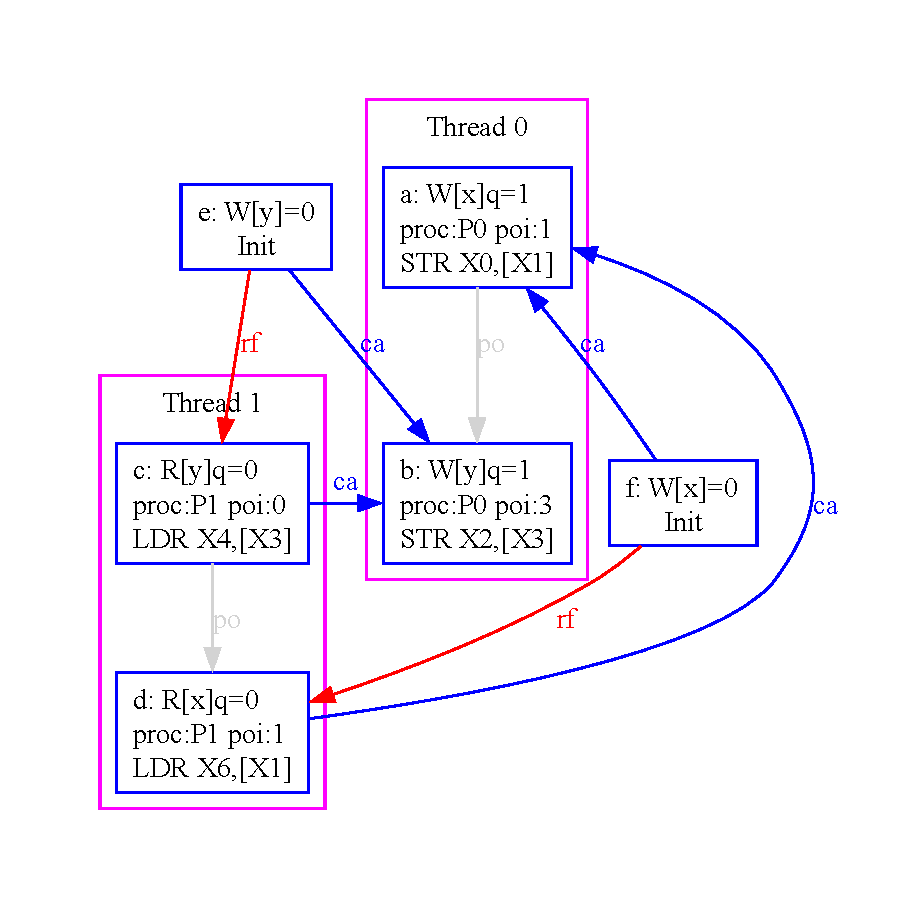
\includegraphics[scale=0.7]{figures/MP-00-crop.pdf}

\vspace{0.5cm}

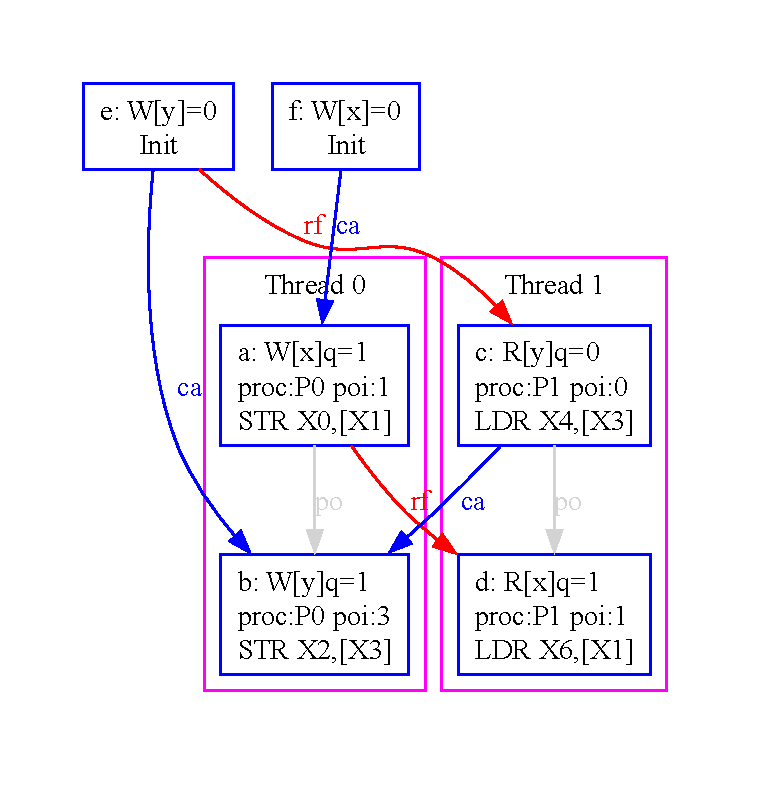
\includegraphics[scale=0.7]{figures/MP-01-crop.pdf}

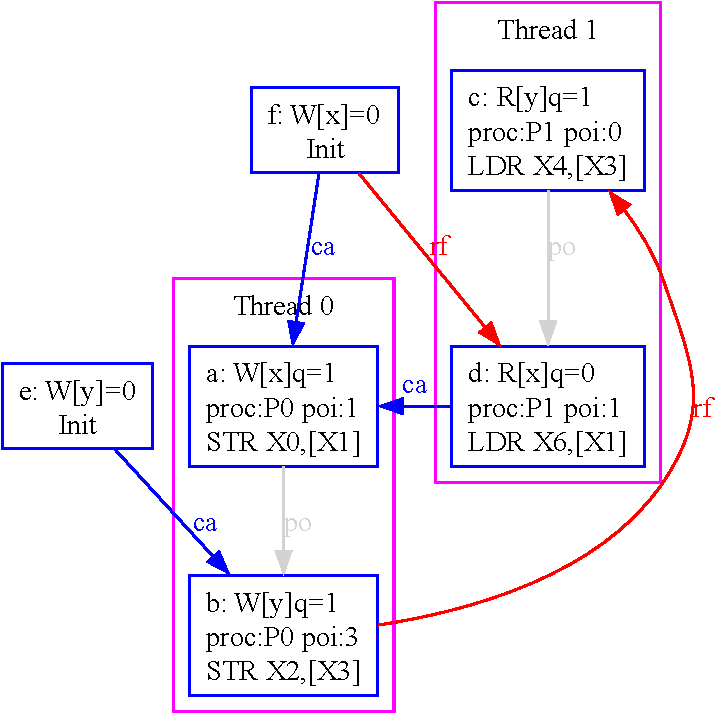
\includegraphics[scale=0.7]{figures/MP-02-crop.pdf}

\vspace{0.5cm}

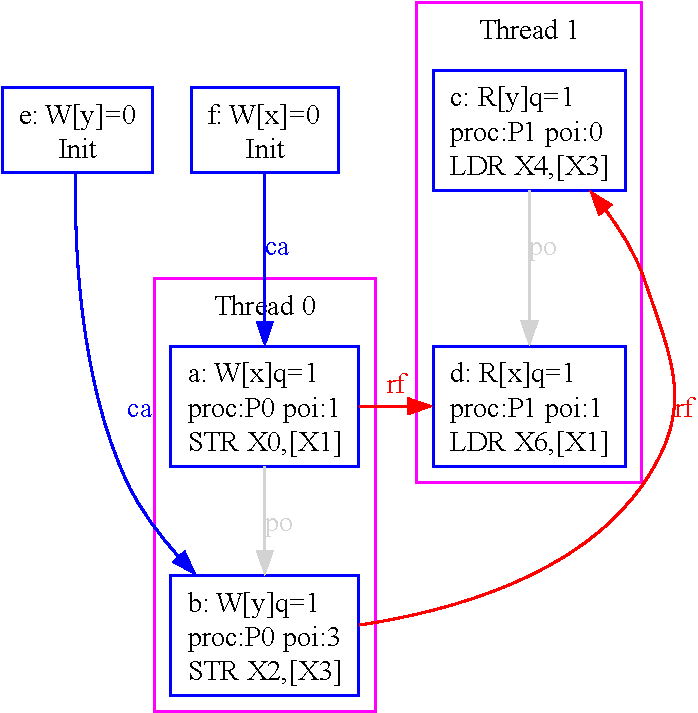
\includegraphics[scale=0.7]{figures/MP-03-crop.pdf}

\newpage

Consider the MP+rel+acq program; it has 3 architecturally Allowed executions, displayed below: 

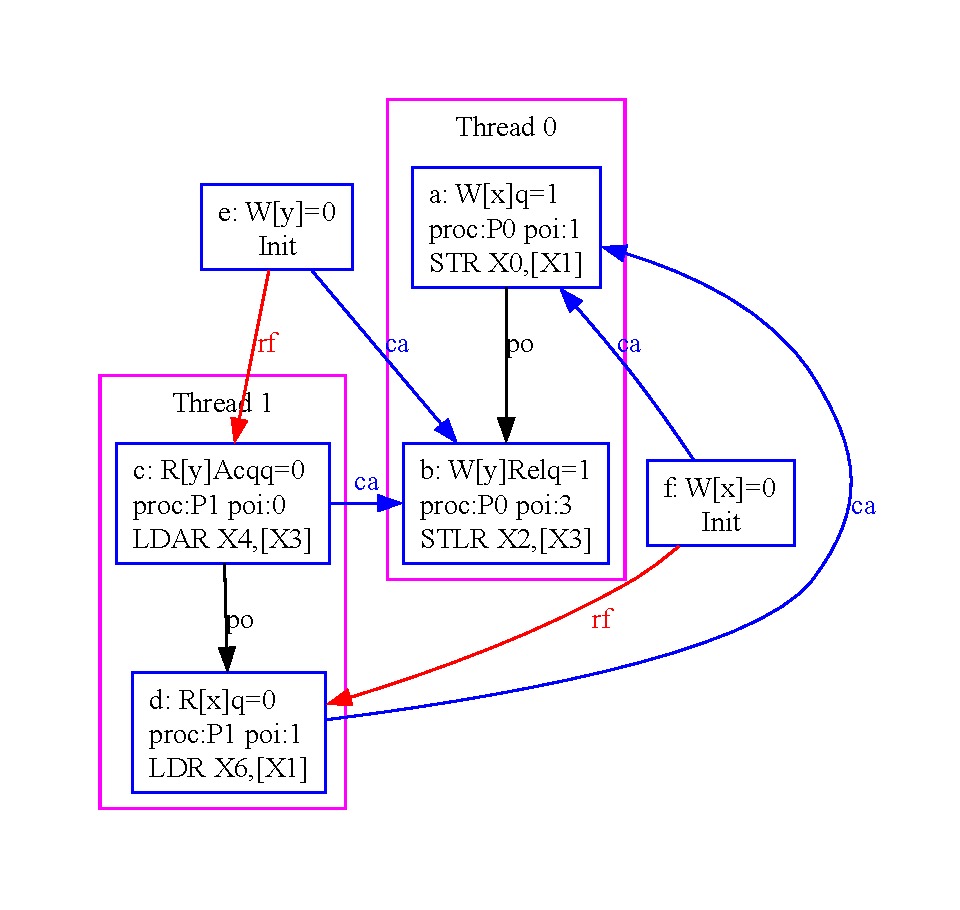
\includegraphics[scale=0.7]{figures/MP+rel+acq-00-crop.pdf}

\vspace{0.5cm}

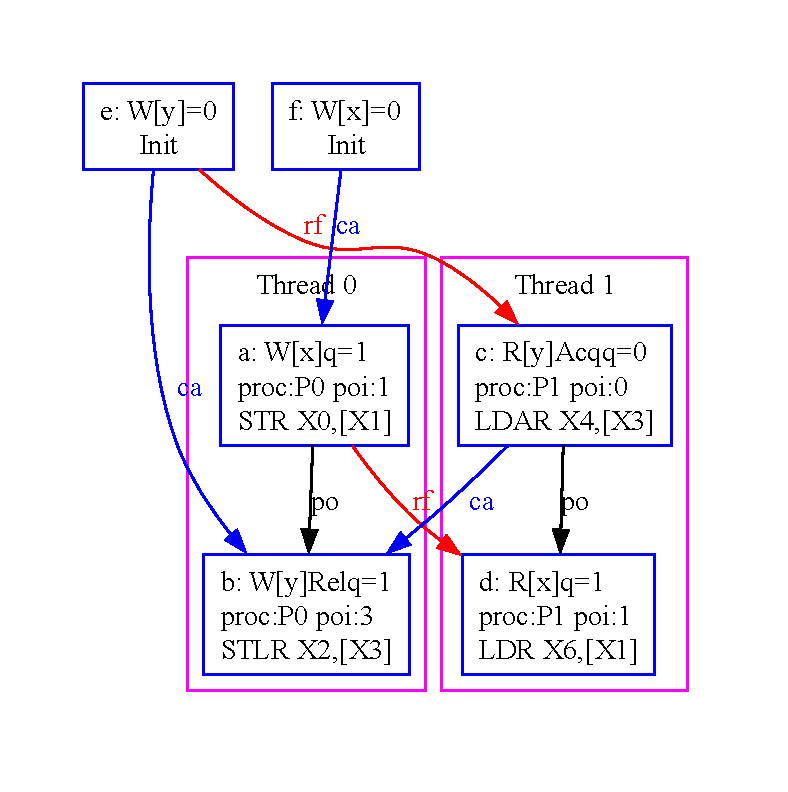
\includegraphics[scale=0.7]{figures/MP+rel+acq-01.pdf}

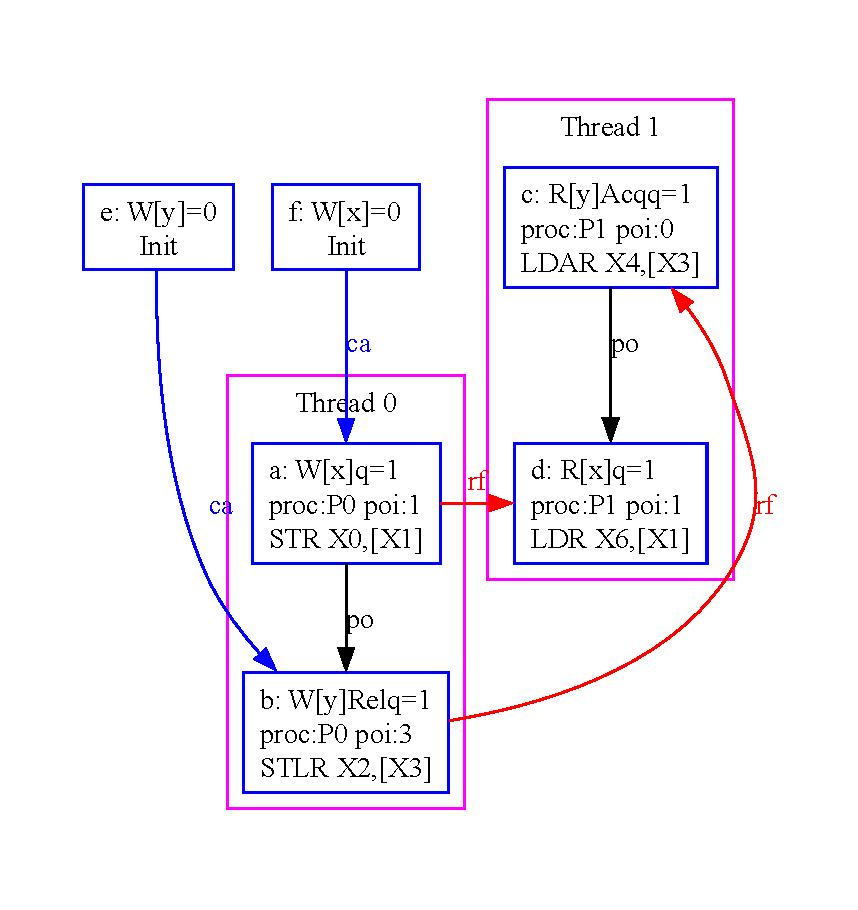
\includegraphics[scale=0.7]{figures/MP+rel+acq-02-crop.pdf}

\vspace{0.3cm}

The rules of the Arm Concurrency Model state
constraints about AArch64 program candidate
executions. Because AArch64 program candidate
executions are described in terms of Effects and
relations between Effects, the Arm Concurrency Model
constraints are necessarily in terms of Effects and
relations between Effects.  
 
The number of Effects to consider, even for one given
instruction, can be quite large. 
%
Indeed one can see the Concurrency Model at different levels of abstraction,
which we sometimes refer to as ``layers of the onion''.  The number and types
of Effects that are relevant at one level, for example at the application level
(intuitively, a level of abstraction where any sort of guard on the way to
physical accesses is assumed to pass, e.g.  translation tables are valid,
memory tags match, etc...), may be rather different to the number and types of
Effects at another level, for example when considering the VMSA.

Typically, at application level, we only need to consider Explicit Memory
Effects, whereas considering the VMSA, instruction fetch, and other features
based on checks or permissions such as MTE, introduces Implicit Memory Effects.
%
Implicit Memory Effects are guards, or checkpoints, on the way to determining
whether an Explicit Memory Effect at application level is permitted to happen,
or if the system should instead fault.

Naturally, the number of relations to grasp and examine can increase too,
depending on the level of abstraction being considered.
%
As a consequence, Arm contributes to the development
of a number of companion tools to help design,
maintain and test its model. Tutorials about these
tools are given here: 
 
\url{https://community.arm.com/arm-community-blogs/b/architectures-and-processors-blog/posts/how-to-use-the-memory-model-tool}

\url{https://community.arm.com/arm-community-blogs/b/architectures-and-processors-blog/posts/generate-litmus-tests-automatically-diy7-tool}

\url{https://community.arm.com/arm-community-blogs/b/architectures-and-processors-blog/posts/running-litmus-tests-on-hardware-litmus7}

\url{https://community.arm.com/arm-community-blogs/b/architectures-and-processors-blog/posts/expanding-memory-model-tools-system-level-architecture}

\section{The domain-specific language ``cat''}

The companion tools to the Arm Concurrency Memory Model are driven by a
domain-specific language called ``cat''. The cat language has a formal syntax
and semantics:  \url{https://arxiv.org/abs/1608.07531}
%
As a consequence, a concurrency model written in cat
is a formal artefact. Therefore, the Arm Concurrency
Model, as represented in cat, is a formal artefact.
The majority of the prose that appears in the Arm ARM
is transliterated from the formal Arm Concurrency
Model written in cat.  
 
The prose in the Arm ARM is not meant to be
machine-readable: users looking for a
machine-readable representation of the Arm
Concurrency Model should turn to the cat file and
process that artefact rather than the prose.
Furthermore, any reinterpretation of the prose of the
Arm ARM which disregards the cat file is liable to
divergence and misinterpretation.  

In cases in which the prose does not appear correct
or is unclear, the cat file should be referenced. If
the intent is still not clear from the cat file,
please contact memory-model@arm.com for clarification
on the intent. 

\section{The ``herd7'' tool}

In addition to being a formal artefact, a concurrency
model written in cat is also an executable artefact.
Indeed, the cat language has been implemented in a
tool called herd7: 
\url{https://developer.arm.com/herd7}

The herd7 tool takes as input a concurrency model
written in cat and a litmus test. Please note that
herd7 is one possible implementation of the cat
language; more precisely, a sound but incomplete
implementation of the cat language: indeed herd7
unrolls loops and cuts them off after a number of
iterations. This is in contrast with the cat language
which is defined over candidate executions in their
full generality, including the cases with potentially
infinite loops. 
 
In summary, whilst the herd7 tool takes as input
litmus tests, the semantics of the cat language
itself is defined over arbitrary programs. In other
words, the formalism described in cat is not limited
to litmus tests, but applies in general to AArch64
programs.  
 
Typically, a litmus test asks whether one specific
candidate execution of a given AArch64 program is
architecturally Allowed or Forbidden, as follows: 
\begin{verbatim}
exists (1:X4=1 /\ 1:X6=0) 
\end{verbatim} 

This asks: “does there exist an architecturally
Allowed execution of the program under scrutiny such
that in the end the register X34 on P1 holds the
value 1 and the register X61 on P1 holds the value
0?”. The answer to this question is yes for MP, but
no for MP+rel+acq. This means that this result is
architecturally Allowed for MP but architecturally
Forbidden for MP+rel+acq. 

Figure~\ref{fig:litmus-mp} shows the complete litmus test for MP.
\litmusinputwithlink[fig:litmus-mp]{MP} 

Figure~\ref{fig:litmus-mp-rel-acq} shows the complete litmus test for MP+rel+acq.
\litmusinputwithlink[fig:litmus-mp-rel-acq]{MP+rel+acq}

Notice the initial state specified between curly
brackets:  
\begin{verbatim}
{ 
0:X1=x; 0:X3=y; 
1:X1=x; 1:X3=y; 
} 
\end{verbatim}

This records the assumptions that initially the
registers X1 on both P0 and P1 hold the address of
some data in the variable x, whilst the registers X3
on both P0 and P1 hold the address of a flag in the
variable y.  
 
When memory locations or registers are not explicitly
initialised, their default initial value is 0. This
is the case in both MP and MP+rel+acq: memory
locations x and y are both initially holding the
value 0. 

\section{Prohibited cycles in candidate executions}

The reason why MP has 4 architecturally Allowed executions whilst MP+rel+acq
only has 3, is that the rules of the Arm Concurrency Model prohibit certain
shapes, called cycles, in the candidate executions of AArch64 programs.
%
For example, the candidate execution of MP+rel+acq shown in
Figure~\ref{fig:mp-rel-acq-forbidden-candidate} is architecturally Forbidden,
as there is a cycle from Effect (a) back to Effect (a), as follows: ``$a
\xrightarrow{po} b \xrightarrow{rf} c \xrightarrow{po} d \xrightarrow{ca} a$''.

\begin{figure}[!htbp]
  \centering
  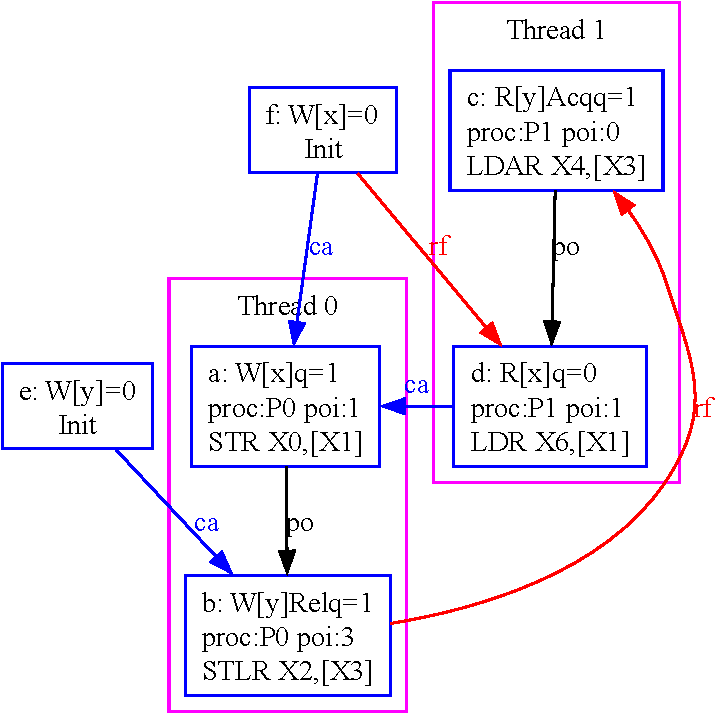
\includegraphics[
    max width=0.7\linewidth
  ]{figures/MP+rel+acq-forbid-crop.pdf}
  \caption{A candidate execution for \texttt{MP+rel+acq}.}
  \label{fig:mp-rel-acq-forbidden-candidate}
\end{figure}

By contrast, the candidate execution of MP shown in
Figure~\ref{fig:mp-02-allowed-candidate} is architecturally Allowed. At first
glance, it might seem like MP exhibits a cycle just like MP+rel+acq does. But
in the case of MP, the cycle ``$a \xrightarrow{po} b \xrightarrow{rf} c
\xrightarrow{po} d \xrightarrow{ca} a$'' is not an architecturally Forbidden
cycle, whereas the cycle in MP+rel+acq is.

\begin{figure}[!htbp]
  \centering
  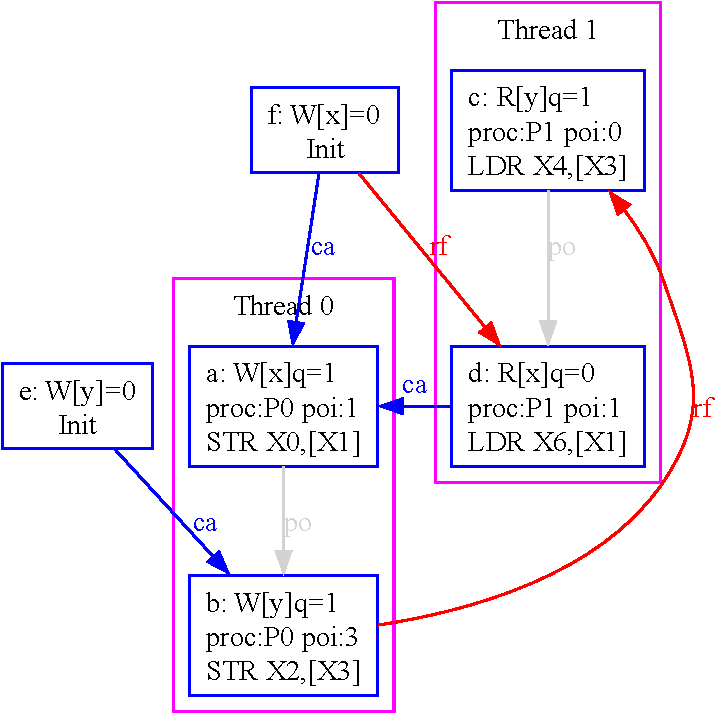
\includegraphics[
    max width=0.7\linewidth
  ]{figures/MP-02-crop.pdf}
  \caption{A candidate execution for \texttt{MP}.}
  \label{fig:mp-02-allowed-candidate}
\end{figure}

The reason for that is that not all cycles are
architecturally Forbidden. Only cycles in an
overarching relation called ``Ordered-before'' are
architecturally Forbidden. In other words,  the rules
of the Arm Concurrency Model prohibit cycles in
``Ordered-before''.  A key part of the concurrency
model is to define which relations contribute to the
Ordered-before relation, and under what
circumstances. 
 
For example, by default, the program order relation
is not included in Ordered-before; intuitively this
means that the Effects generated by two instructions
in program order can be reordered by a PE, unless
otherwise stated. To help see this better in the
graphs, the program order arrows are depicted in
light grey by default, unless there is an
architectural requirement for a specific program
order arrow to maintain order, in which case the
program order arrows are depicted in black. 

This is the case in MP+rel+acq. In MP+rel+acq, the
program order arrow on P0 (resp. P1) are required to
maintain order: this is due to the presence of the
annotation ``Rel'' (resp. Acq) on the Explicit Memory
Write Effect (b) on P0 (resp. Effect (c) on P1),
which come from the fact that Effect (b) (resp.
Effect (c)) is generated by a Store-Release STLR
(resp. Load-Acquire LDAR) instruction.

\section{Relations included in ``Ordered-before''}

The Arm Concurrency Model mandates  which relations of an AArch64 program
candidate execution must be included in Ordered-before. For a given AArch64
program candidate execution, some of its relations are required to be included
in Ordered-before, and others are not.  

\begin{figure}[!htbp]
  \centering
  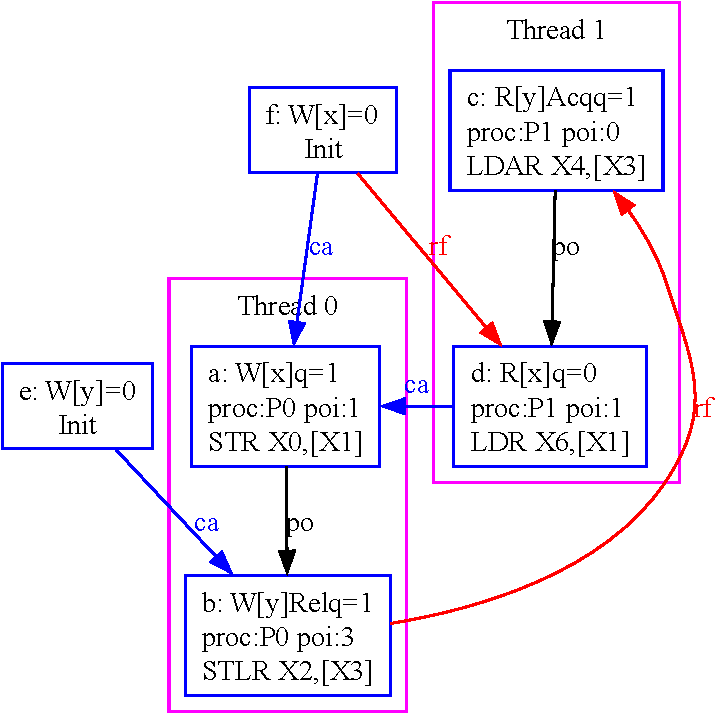
\includegraphics[
    max width=0.7\linewidth
  ]{figures/MP+rel+acq-forbid-crop.pdf}
  \caption{A candidate execution for \texttt{MP+rel+acq}.}
  \label{fig:mp-rel-acq-ob-candidate}
\end{figure}

For example, in MP+rel+acq, Figure~\ref{fig:mp-rel-acq-ob-candidate} shows a
candidate execution where program order contributes to Ordered-before.
%
The program order relation on P0 between the Explicit
Memory Write Effect (a) and the Explicit Memory Write
Effect (b) is required to be included in
Ordered-before. The reason for this is that the
Explicit Memory Write Effect (b) is generated by a
Store Release instruction (notice the Rel annotation
on Effect (b)).  
 
Similarly, the program order relation on P1 between
the Explicit Memory Read Effect (c) and the Explicit
Memory Read Effect (d) is required to be included in
Ordered-before. The reason for this is that the
Explicit Memory Read Effect (c) is generated by a
Load Acquire instruction (as denoted by the Acq
annotation on Effect (c)). 

\begin{figure}[!htbp]
  \centering
  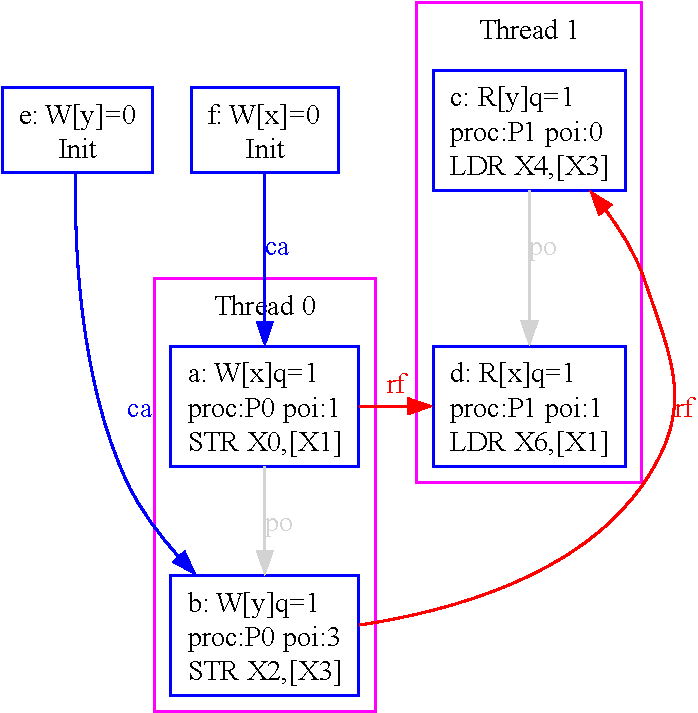
\includegraphics[
    max width=0.7\linewidth
  ]{figures/MP-03-crop.pdf}
  \caption{A candidate execution for \texttt{MP}.}
  \label{fig:mp-03-ob-candidate}
\end{figure}

By contrast, Figure~\ref{fig:mp-03-ob-candidate} shows a candidate execution
for MP.
%
The program order relation on P0 between the Explicit
Memory Write Effect (a) and the Explicit Memory Write
Effect (b) is not required to be included in
Ordered-before. This is because, unlike in
MP+rel+acq, the Explicit Memory Write Effect (b) is
not generated by a Store Release instruction, and
there is no other means of ordering present on P0.  
 
Similarly, the program order relation on P1 between
the Explicit Memory Read Effect (c) and the Explicit
Memory Read Effect (d) is not required to be included
in Ordered-before. This is because, unlike in
MP+rel+acq, the Explicit Memory Read Effect (c) is
not generated by a Load Acquire instruction and there
is not other means of ordering present on P1.

\section{Cycles in the ``Ordered-before'' relation}

The Arm Concurrency Model prohibits cycles in the “Ordered-before” relation.
Mathematically, a relation which is acyclic is called
an order: in other words, a relation which can be
relied on to order elements in its domain of
definition (i.e. the extremities of the arrows
depicting that relation). In turn this means that a
relation which is acyclic can be reasoned about more
intuitively than one that is cyclic. Indeed, there
are a number of orders which we rely on intuitively,
e.g. “less than” over natural numbers, the alphabet,
or coordinates. 
 
The Arm Concurrency Model requires the Ordered-before
relation to be acyclic. This means that
Ordered-before can be relied upon as a way to order
Memory Effects. Sometimes this is referred to as
preventing the absence of ``causal loops''---such loops
hinder reasoning.  
 
For example, Figure~\ref{fig:mp-rel-acq-acyclicity-candidate} shows the
candidate execution for MP+rel+acq.

\begin{figure}[!htbp]
  \centering
  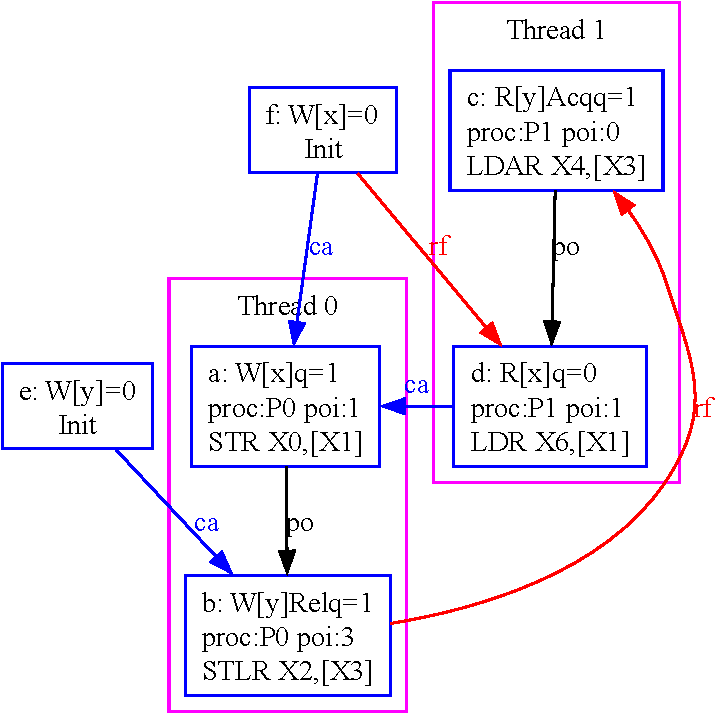
\includegraphics[
    max width=0.7\linewidth
  ]{figures/MP+rel+acq-forbid-crop.pdf}
  \caption{A candidate execution for \texttt{MP+rel+acq}.}
  \label{fig:mp-rel-acq-acyclicity-candidate}
\end{figure}

As mentioned above, the program order relations
between Explicit Memory Write Effects (a) and (b) on
P0 (resp. Explicit Memory Read Effects (c) and (d) on
P1) are required to be included in Ordered-before,
due to b being generated by a Store Release (resp. c
being generated by a Load Acquire). 
 
Additionally, the Reads-from relation between Effects
generated by different PEs is also required to be
included in Ordered-before. In the candidate
execution of MP+rel+acq shown in
Figure~\ref{fig:mp-rel-acq-acyclicity-candidate}, this is the case for
the Reads-from relation between the Explicit Memory
Write Effect (b) on P0 and the Explicit Memory Read
Effect (c) on P1. 
 
Finally, the Coherence-after relation between Effects
generated by different PEs is also required to be
included in Ordered-before. In the candidate
execution of MP+rel+acq shown in
Figure~\ref{fig:mp-rel-acq-acyclicity-candidate}, this is the case for
the Coherence-after relation between the Explicit
Memory Read Effect (d) on P1 and the Explicit Memory
Write Effect (a) on P0. 
 
All in all this means that the candidate  execution
of MP+rel+acq exhibits a cycle in Ordered-before: “$a
\xrightarrow{po} b \xrightarrow{rf} c \xrightarrow{po} d \xrightarrow{ca} a$”, which means that
this candidate execution is architecturally
Forbidden. 

By contrast, Figure~\ref{fig:mp-03-acyclicity-candidate} shows the candidate
execution for MP.

\begin{figure}[!htbp]
  \centering
  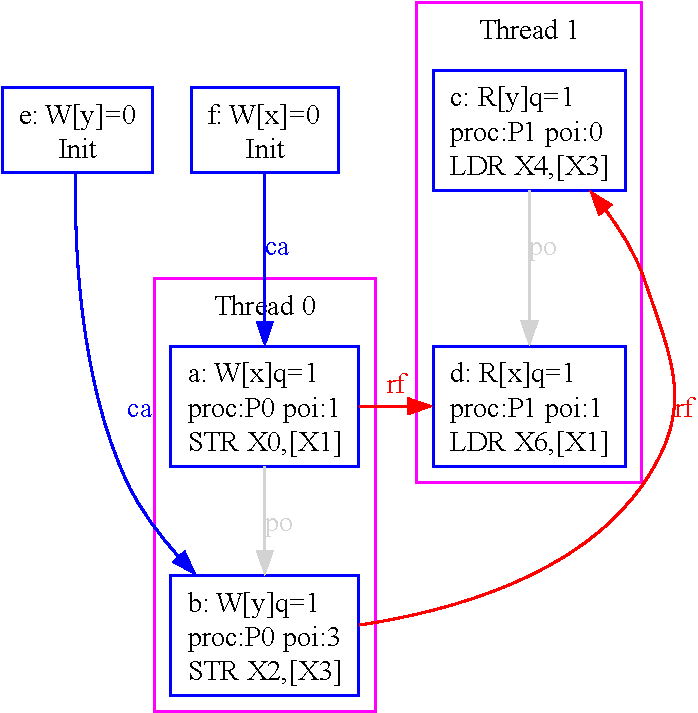
\includegraphics[
    max width=0.7\linewidth
  ]{figures/MP-03-crop.pdf}
  \caption{A candidate execution for \texttt{MP}.}
  \label{fig:mp-03-acyclicity-candidate}
\end{figure}

The program order relations in both P0 and P1 are not
required to be included in Ordered-before; as a
consequence this candidate execution of MP does not
exhibit a cycle in Ordered-before and is therefore
architecturally Allowed. 

\section{Taxonomy of requirements over relations}

To help users of the Concurrency Model navigate its
definition, Arm organises relations depending on
their significance. 
%
In other words, Arm aims to provide a taxonomy of
requirements over these relations depending on their
significance to hardware, e.g. to help determine
which relation is of importance when designing:  
\begin{itemize}
\item a single core, or  
\item the machinery outside the core to provide
ordering guarantees across multiple cores.
\end{itemize}

This taxonomy also might be of use when examining these relations from a software point of view. 
 
Overall, requirements on hardware are as follows---the remainder of this note details each concept in turn: 
\begin{itemize}
\item In Section~\ref{sec:instr-sem-reqs}, we discuss Instruction semantics
requirements, namely the definitions of Intrinsic dependencies ``iico\_data'',
``iico\_ctrl'' and ``iico\_order'' in cat, and how these relations are used to
build other relations, for example Address, Data or Control dependencies at the
AArch64 level; 

\item In Section~\ref{sec:internal-visibility-reqs}, we discuss Internal
visibility requirements, namely the axioms called ``coRW1-Exp'', ``coWW-Exp''
and ``coWR-Exp'' in the cat file; these impose a requirement on hardware to
provide Architecturally valid values;   

\item In Section~\ref{sec:external-visibility-reqs}, we discuss External
visibility requirement: namely the ``external'' axiom in the cat file; this
imposes a requirement on hardware to provide order between the Effects that are
related by a relation included in Ordered-before;  

\item In Section~\ref{sec:atomicity-req}, we discuss the Atomicity requirement:
  namely the ``atomic'' axiom in the cat file; this imposes a requirement on
    hardware to provide the appearance of atomicity between Effects that come
    from, for example, a successful Load-Exclusive/Store-Exclusive pair,  or a
    CAS.
\end{itemize}

The remainder of this note details these requirements one by one. 

\section{Instruction semantics requirements \label{sec:instr-sem-reqs}}

Intrinsic Dependencies stem from, and are hardware requirements on, the semantics of a
given AArch64 instruction. In the Arm ARM, the
semantics of an instruction is given by its ASL code.  
Much like the program order at the AArch64 level does
not necessarily provide order, the order of
statements in the ASL code of an instruction does not
necessarily provide order between the different
statements that define that instruction. In other
words, the ASL semicolon ``;'' does not provide order
in the general case. Instead, there are 3 mechanisms,
called Intrinsic dependencies, that do create order
between ASL statements.  
 
Intrinsic dependencies can be: 
\begin{itemize}
\item Intrinsic Data Dependencies; 
\item Intrinsic Control Dependencies; 
\item Intrinsic Order Dependencies. 
\end{itemize}
 
In all 3 cases, an Intrinsic Dependency relation only
exists between Effects of a sole AArch64 instruction.
In other words, Intrinsic Dependencies do not relate
Effects from different instructions. 
 
Arm has been formalising the semantics of the ASL
language. This formalisation work enables Arm to
provide a precise, formal definition of when the
instruction semantics of an instruction, as described
by the ASL code of that instruction, indicates the
presence of an Intrinsic dependency of whichever
nature: Data, Control, or Order. 

Intuively, Intrinsic Data Dependencies can
be determined by the data flow of the ASL code, and
Intrinsic Control Dependencies can be
determined by the control flow of the ASL code.

In most cases, with the ASL corpus as it is today, it is possible to infer
Intrinsic Data Dependencies and Intrinsic Control Dependencies from the ASL
code of an instruction, but it is not universally the case today: Arm is
currently working to ensure that this property holds true throughout the ASL
corpus.  Historical discrepancies include the code of CAS, which has now been
adjusted. 

\subsection{Intrinsic Data Dependencies}
 
Intuitively, for a given AArch64 instruction I
generating Effects E1 and E2, an Intrinsic Data
Dependency from an Effect E1 to an Effect E2
indicates that E1 transmits some data necessary to
the operation of I to E2. 
 
Consider the semantics of a load instruction LDR
X1,[X0], where register X0 points to the address x,
and x initially holds the value 42. 

At the application level, LDR X1,[X0] operates as follows:

\begin{enumerate}
\item Read register X0, obtain address x; 
\item Read address x, obtain value 42; 
\item Write value 42 into register X1. 
\end{enumerate}

Going from step 1 to step 2 necessitates transmitting
some information, namely the address x. Similarly
going from step 2 to step 3 necessitates transmitting
some information, namely the value 42. 

\begin{figure}[!htbp]
  \centering
  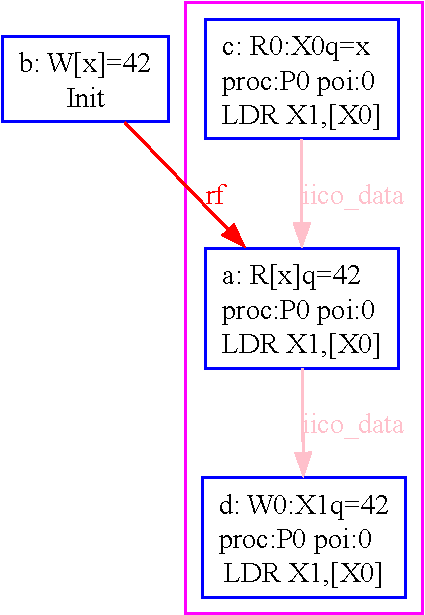
\includegraphics[
    max width=0.5\linewidth,
    max totalheight=0.35\textheight
  ]{figures/LDR-crop.pdf}
  \caption{Application-level semantics for \texttt{LDR X1,[X0]}.}
  \label{fig:ldr-instruction-semantics}
\end{figure}

Figure~\ref{fig:ldr-instruction-semantics} shows this graphically: Effect (c) corresponds to step 1. Effect (a) corresponds to step 2. Effect (d) corresponds to step 3. The arrows labelled “iico\_data” depict Intrinsic data dependencies, and represent the transmission of information from one Effect to the next. 
The semantics of LDR shown in Figure~\ref{fig:ldr-instruction-semantics} is
very sequential: the Effects cannot occur in parallel as each one transmits some
information to the next. These Intrinsic Data dependencies impose some
requirements on the hardware to ensure that LDR X1,[X0] operates as intended.
 
By contrast, consider the semantics of a store instruction STR X2,[X0], where register X0 points to address x and register X2 holds the value 7. At the application level, STR X2,[X0] operates as follows: 
\begin{itemize}
\item[1a.] Read register X0, obtain address X 
\item[1b.]  Read register X2, obtain value 7 
\item[2.] Write value 7 into x 
\end{itemize}

It is not necessary to perform step 1a and step 1b in sequence: they can be done in either order, or indeed in parallel. 

\begin{figure}[!htbp]
  \centering
  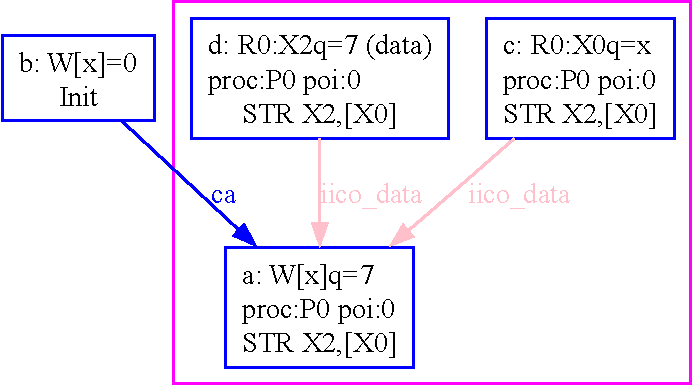
\includegraphics[
    max width=0.7\linewidth
  ]{figures/STR-crop.pdf}
  \caption{Application-level semantics for \texttt{STR X2,[X0]}.}
  \label{fig:str-instruction-semantics}
\end{figure}

Figure~\ref{fig:str-instruction-semantics} shows this graphically: Effect (c)
corresponds to step 1a. Effect (d) corresponds to step 1. Effect (a)
corresponds to step 2.
%
There is an Intrinsic Data dependency from Effect (c)
to Effect (a), corresponding to the transmission of
the address x. There is an Intrinsic Data dependency
from Effect (d) to Effect (a), corresponding to the
transmission of the value 7. These Intrinsic Data
dependencies impose some requirements on the hardware
to ensure that STR X2,[X0] operates as intended. 
 
There is no dependency between Effect (d) and Effect
(c), corresponding to the fact that it is not
necessary to perform step1 and step 1bis in sequence.
This means that the hardware is not required to order
Effect (c) and Effect (d), or in other words,
hardware is free to execute these Effects in either
order or in parallel. 

\subsection{Intrinsic Control Dependencies}

Intuitively, for a given AArch64 instruction I
generating Effects E1 and E2, there is an Intrinsic
Control Dependency from an Effect E1 to an Effect E2
if and only if all the following apply:
\begin{itemize}
\item E1 is an Intrinsic Branching Effect, or in
other words, a decision point within the semantics of
instruction I (or the control flow of its ASL code);
\item The instruction semantics for that instruction I
indicate that the generation of E2 depends on the
condition determination of E1. 
\end{itemize}

Consider the semantics of a load instruction LDR X1,[X2], at VMSA level, where
register X2 points to the virtual address x, initially x holds the value 42,
and the Translation Table Descriptor of x, namely TTD(x), is initially invalid
(in other words, its valid bit is 0). 

At the VMSA level, LDR X1,[X2] operates as follows: 
\begin{enumerate}
\item Read address register X2, obtain virtual address x; 
\item Read the Translation Table Descriptor of x, namely TTD(x); 
\item Make a decision depending on the value of TTD(x); 
\item If the TTD(x) is invalid, as is the case here: 
\begin{itemize}
\item Write to ELR\_EL1; 
\item Generate a Fault.
\end{itemize} 
\end{enumerate}
 
Going from step 1 to step 2 necessitates transmitting
some information, namely the address x. Similarly
going from step 2 to step 3 necessitates transmitting
some information, namely the value of TTD(x). Thus
there are Intrinsic Data dependencies from the Effect
corresponding to step 1 to the Effect corresponding
to step 2, and from the Effect corresponding to step
2 to the Effect corresponding to step 3.  
%
Going from step 3 to either substep of step 4
corresponds to an Intrinsic Control dependency, since
the substeps of step 4 depend on the condition
determination of step 3. 
%
Figure~\ref{fig:ldrv0-instruction-semantics} shows this graphically.

\begin{figure}[!htbp]
  \centering
  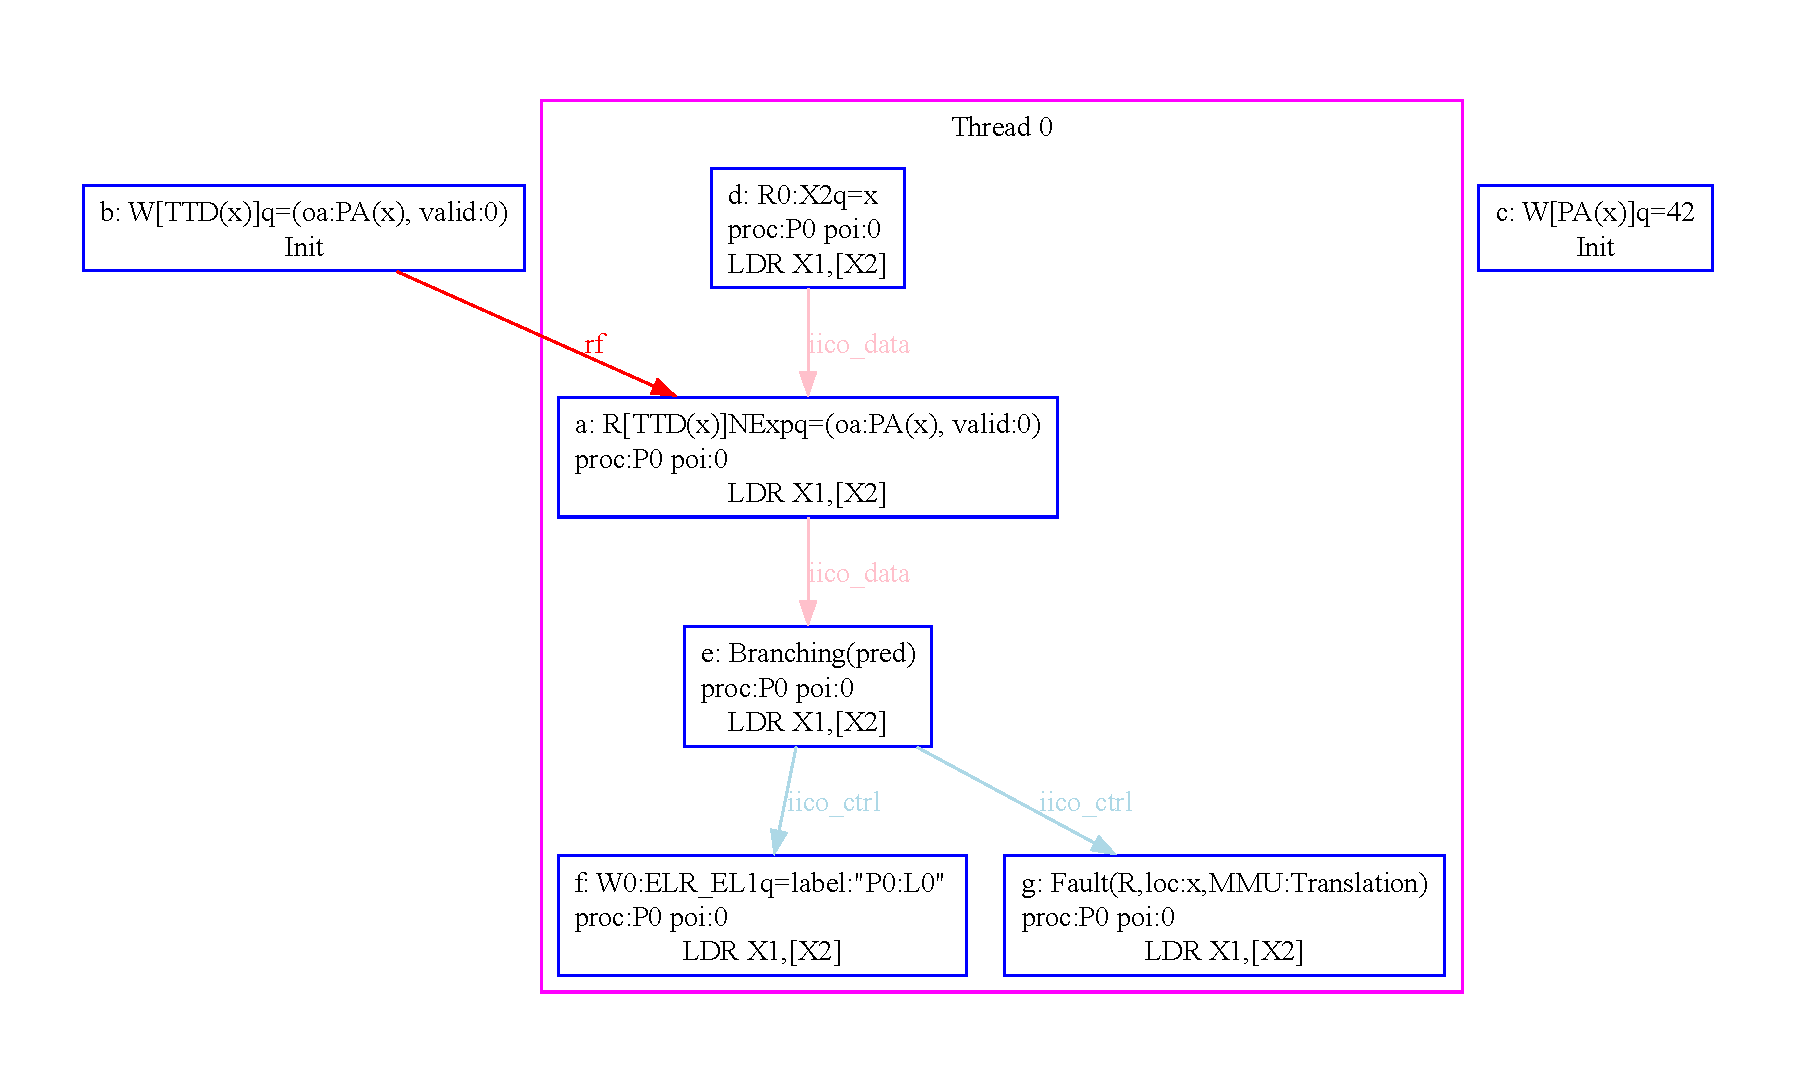
\includegraphics[
    max width=\linewidth
  ]{figures/LDRv0-crop.pdf}
  \caption{Application-level semantics for \texttt{LDR X1,[X0]} when the TTD of
  \texttt{x} is invalid.}
  \label{fig:ldrv0-instruction-semantics}
\end{figure}

In the case where the TTD of x is initially valid,
the semantics becomes as shown in
Figure~\ref{fig:ldrv1-instruction-semantics}.
%
In this case, the instruction does not fault since
the TTD is valid. Instead, the instruction generates
an Explicit Memory Read Effect of the corresponding
PA: this is Effect (b). There still is an Intrinsic
Control dependency from the decision point (Effect
(f)) to the Explicit Memory Read Effect (b). 


\begin{figure}[!htbp]
  \centering
  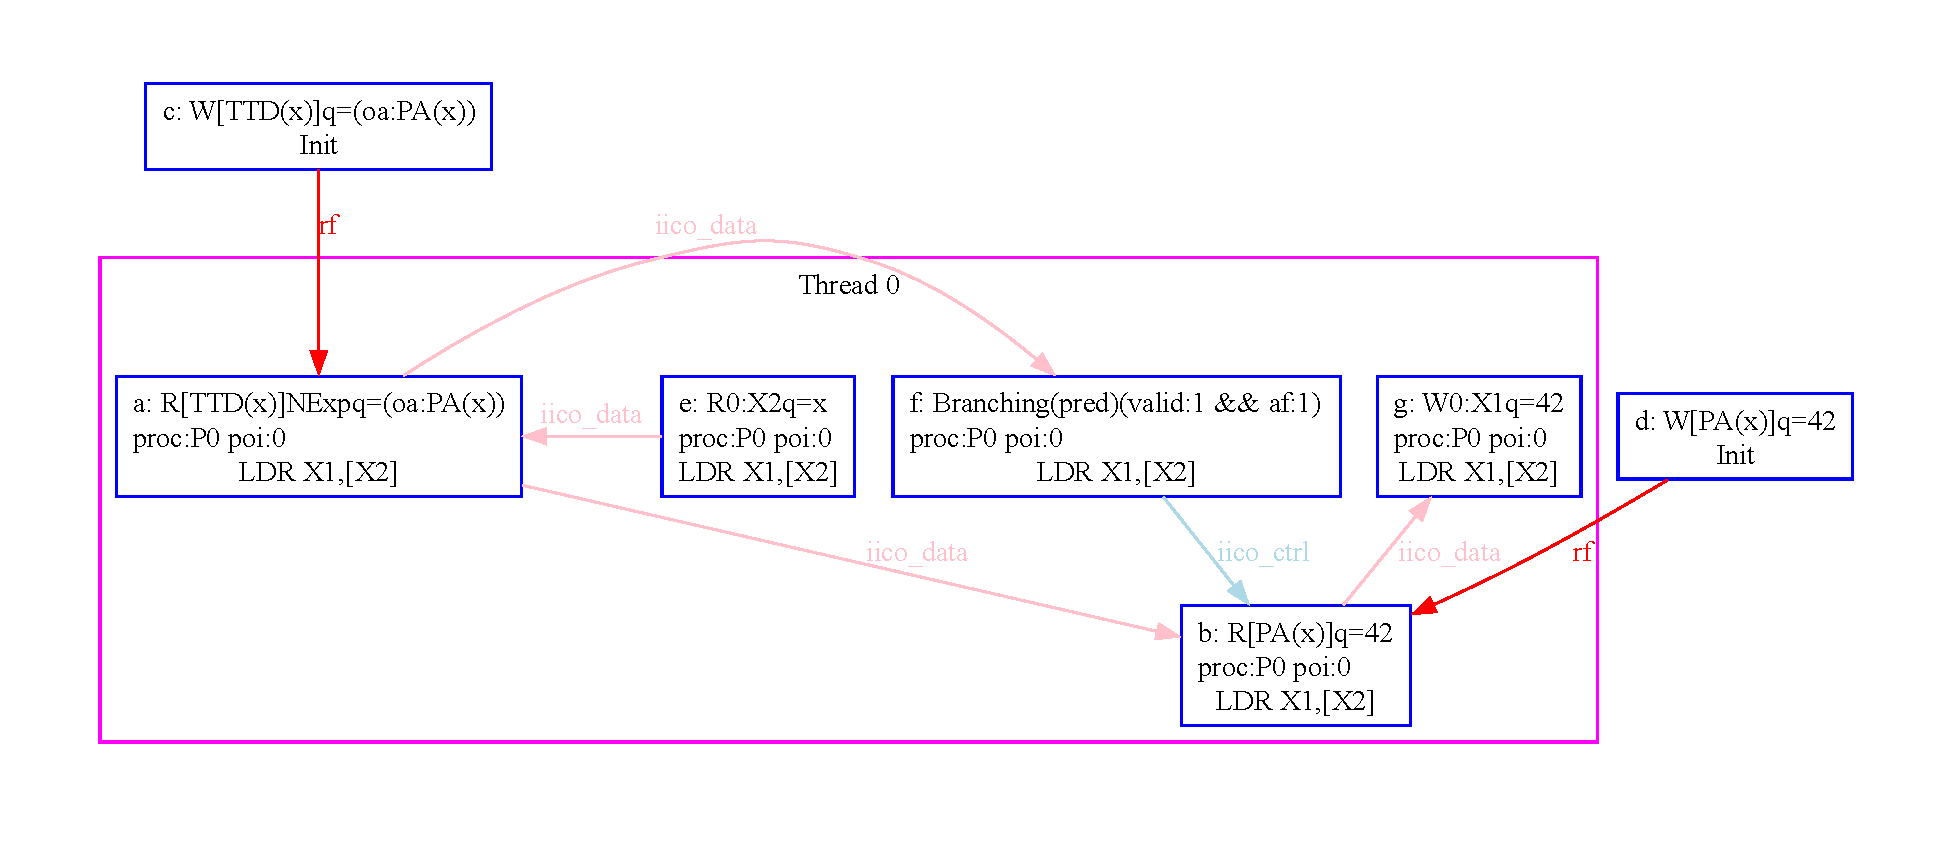
\includegraphics[
    max width=\linewidth
  ]{figures/LDRv1-crop.pdf}
  \caption{Application-level semantics for \texttt{LDR X1,[X0]} when the TTD of
  \texttt{x} is valid.}
  \label{fig:ldrv1-instruction-semantics}
\end{figure}

\subsection{Intrinsic Order Dependencies}

Intuitively, for a given AArch64 instruction I
generating Effects E1 and E2, an Intrinsic Order
Dependency from an Effect E1 to an Effect E2
indicates that the architecture prescribes that E1 is
Ordered-before E2, even though the instruction
semantics of I, as described in the ASL code of the
instruction I, do not appear to mandate this
ordering.  
%
In other words, Intrinsic Order dependencies are
Intrinsic dependencies that are mandated by the
architecture for additional purposes to the
computational aspect of the instruction.  

Currently intrinsic order dependencies are only
expressed in prose, as this requirement cannot be
made through the data flow or control flow of the ASL
code.
%
Arm intends to extend the ASL language with a
syntactic construct to signify the presence of an
Intrinsic Order dependency from within the ASL code
of an instruction. 

Examples of occurrences of Intrinsic Order
dependencies include: 
\begin{itemize}
\item The two Explicit Memory Write Effects of STILP; 
\item The two Explicit Memory Read Effects of LDIAPP; 
\item The Explicit Memory Effects of SWP; 
\item The Effects of certain vector instructions. 
\end{itemize} 

Consider the semantics of a load instruction LDIAPP
W0,W1,[X2], where register X2 points to the address
x, and the array x[] initially holds the value {0,0},
or in other words x holds the value 0 and x+4 holds
the value 0. 
%
At the application level, LDIAPP W0,W1,[X2] operates as
follows: 
\begin{itemize}
\item[1.] Read address register X2, obtain address x; 
\item[2.] Read address x, obtain value 0; 
\item[2bis.] Read address x+4, obtain value 0; 
\item[3.] Write value 0 obtained from x into data register X0; 
\item[3bis.] Write value 0 obtained from x+4 into data register X1. 
\end{itemize}

In addition to these necessary functional steps, the architecture mandates that
steps 2 and 2bis should be done in sequence. This is because LDIAPP was
designed to provide a stronger ordering semantics than its plain sibling LDP:
LDIAPP provides AcquirePC semantics to the Load. 

Figure~\ref{fig:ldiapp-intrinsic-order-semantics} shows this graphically.
Observe the Intrinsic Order dependency from the Explicit Memory Read Effect (a)
of x and the Explicit Memory Read Effect (b) of x+4, namely, the iico\_order
arrow from Effect (a) to Effect (b).

\begin{figure}[!htbp]
  \centering
  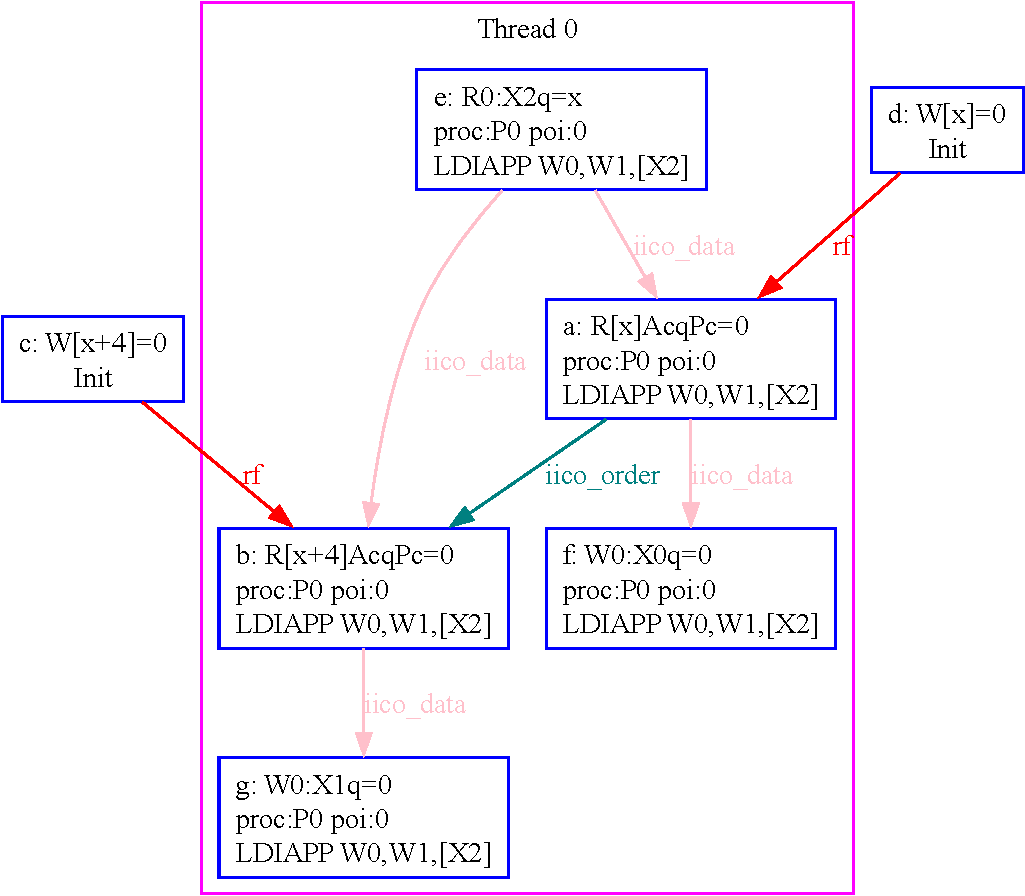
\includegraphics[
    max width=0.8\linewidth
  ]{figures/LDIAPP-crop.pdf}
  \caption{Application-level semantics for \texttt{LDIAPP W0,W1,[X2]}.}
  \label{fig:ldiapp-intrinsic-order-semantics}
\end{figure}

To simply perform a Load-pair, it is unnecessary to order the Explicit Memory Read Effect (a) of x and the Explicit Memory Read Effect (b) of x+4, or in other words, in requiring that steps 2 and 2bis should be done in sequence.  
 
Indeed the semantics of a plain LDP does not mandate
an Intrinsic Order dependency between the two
corresponding Effects, or steps: in the instruction
semantics diagram of LDP shown in
Figure~\ref{fig:ldp-intrinsic-order-semantics}, there is no Intrinsic Order
dependency, namely, no iico\_order arrow from Effect (a) to Effect (b).

\begin{figure}[!htbp]
  \centering
  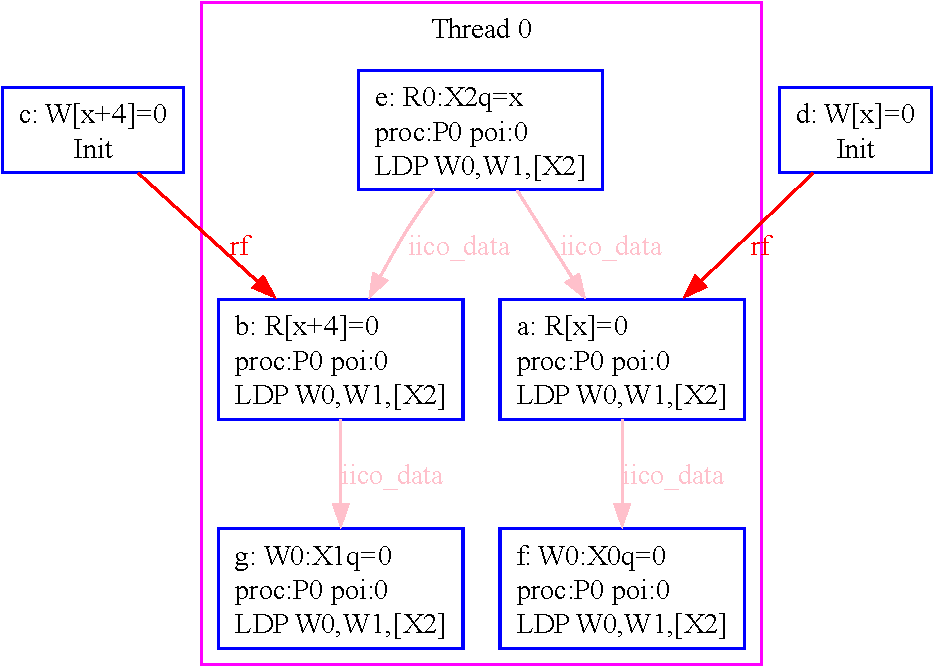
\includegraphics[
    max width=0.8\linewidth
  ]{figures/LDP-crop.pdf}
  \caption{Application-level semantics for \texttt{LDP W0,W1,[X2]}.}
  \label{fig:ldp-intrinsic-order-semantics}
\end{figure}

Similarly in the store case, the semantics of an
STILP mandates an Intrinsic Order dependency between
its two Explicit Memory Write Effects. 
%
More precisely, if X2 holds the address x, STILP
W0,W1,[X2] would require an Intrinsic dependency from
the Explicit Memory Write Effect of x to the Explicit
Memory Write Effect of x+4.
%
This is in contrast with a plain STP which does not
mandate any ordering between its Explicit Memory
Write Effects. Figure~\ref{fig:stilp-intrinsic-order-semantics} shows this.

\begin{figure}[!htbp]
  \centering
  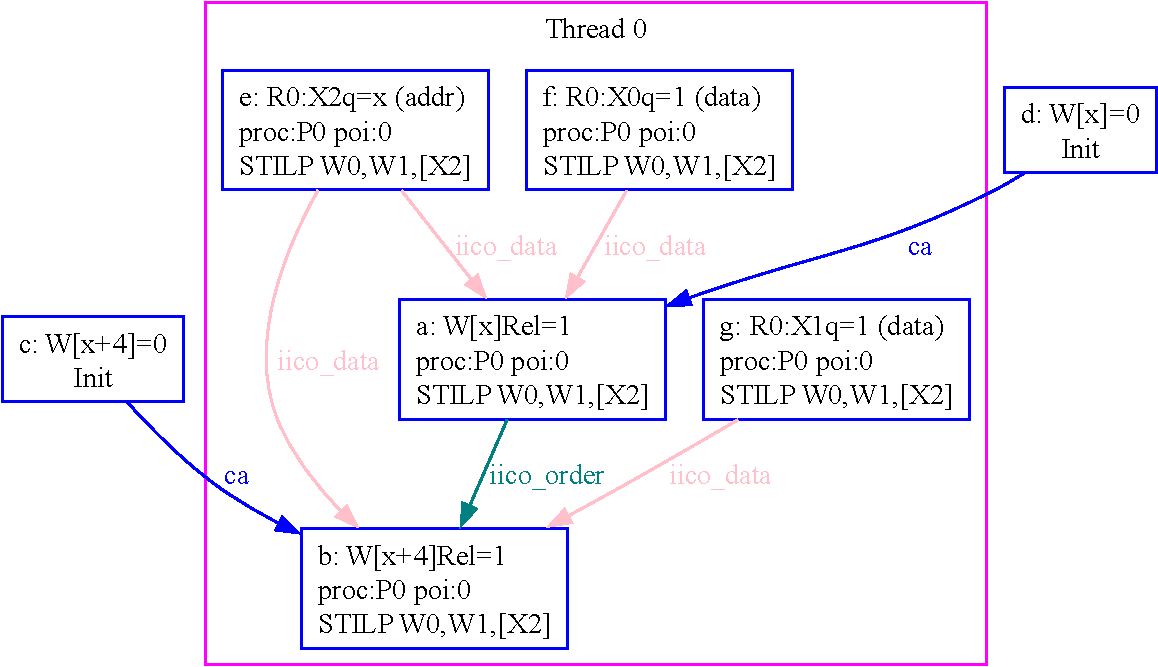
\includegraphics[
    max width=0.8\linewidth
  ]{figures/STILP-crop.pdf}
  \caption{Application-level semantics for \texttt{STILP W0,W1,[X2]}.}
  \label{fig:stilp-intrinsic-order-semantics}
\end{figure}

Certain Intrinsic Order dependencies are included in
Ordered-before. This can lead to certain program
candidate executions being architecturally Forbidden.
This is the case of the Intrinsic Order dependencies
created by STILP and LDIAPP. 

Consider the litmus test in Figure~\ref{fig:litmus-mp-dmb-st-ldiapp}, which involves LDIAPP.
\litmusinputwithlink[fig:litmus-mp-dmb-st-ldiapp]{MP+dmb.st+LDIAPP}

This test asks whether the following candidate execution is architecturally Allowed: 
\begin{itemize}
\item the Explicit Memory Read Effect of x generated
by LDIAPP on P1 reads from the Explicit Memory Write
Effect of x generated by the first STR on P0;
\item the Explicit Memory Read Effect of x+4
generated by LDIAPP on P1 does not read from the
Explicit Memory Write Effect of x+4 generated by
STR on P0, taking its value from the initial state
of x+4 instead. 
\end{itemize}

\begin{figure}[!htbp]
  \centering
  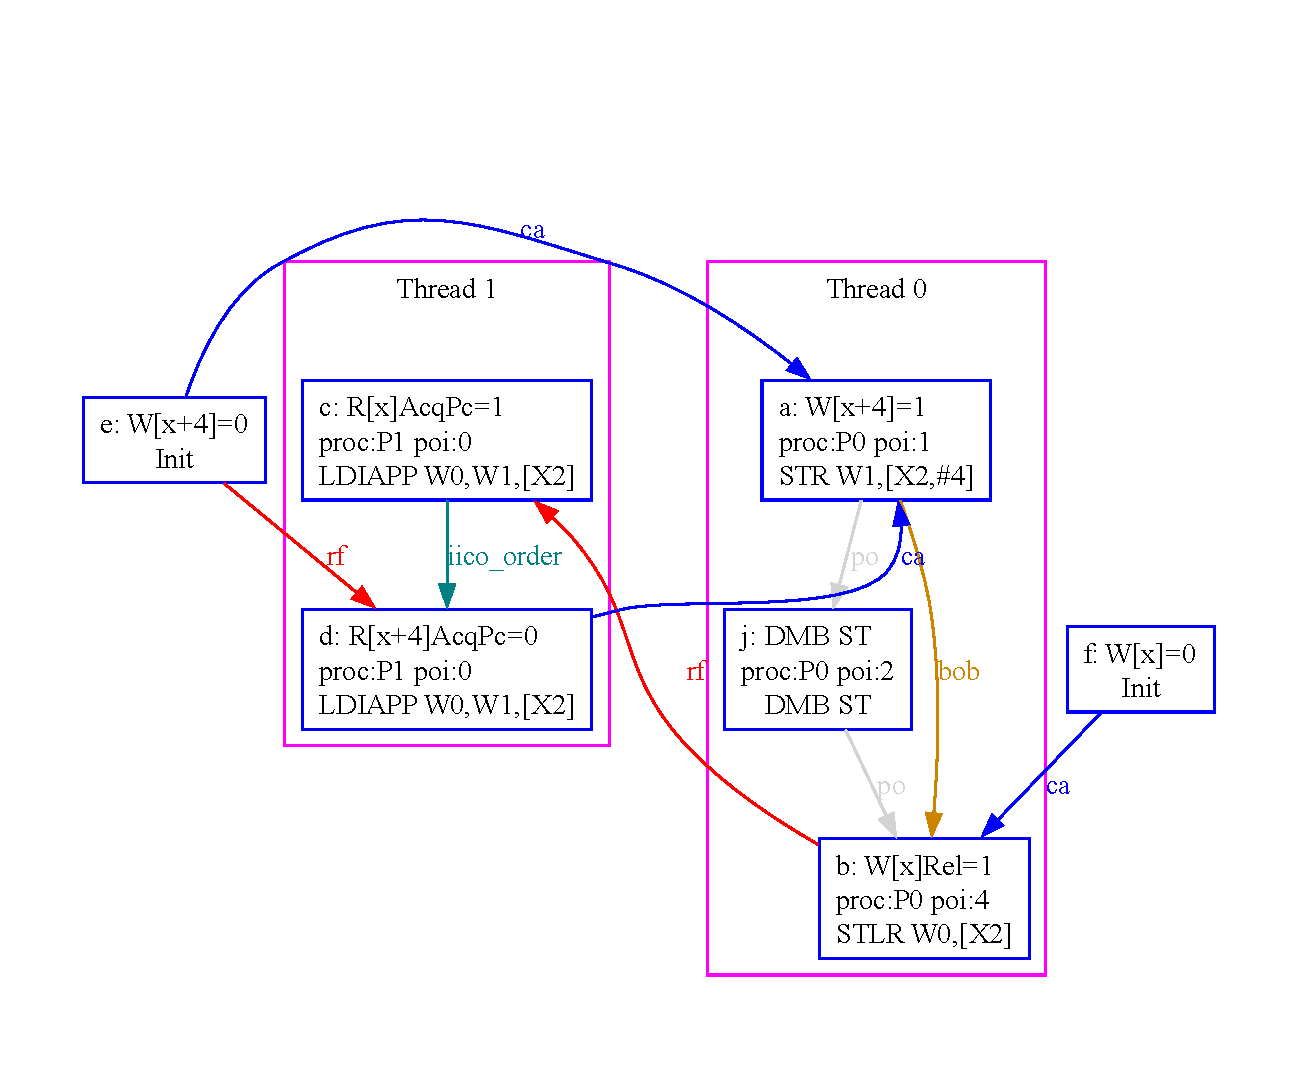
\includegraphics[
    max width=0.8\linewidth
  ]{figures/MP+dmb.st+LDIAPP-crop.pdf}
  \caption{A candidate execution for \texttt{MP+dmb.st+LDIAPP}.}
  \label{fig:mp-dmb-st-ldiapp-candidate}
\end{figure}

Figure~\ref{fig:mp-dmb-st-ldiapp-candidate} shows this graphically.
%
This candidate execution is architecturally Forbidden, due to:
\begin{itemize}
\item The Intrinsic Order Dependency between The Explicit Memory Read Effect of
  x (c) and the Explicit Memory Read Effect of x+4 (d) generated by LDIAPP on P1;
\end{itemize}
combined with:
\begin{itemize}
\item The fact that the Explicit Memory Read Effect
of x+4 (d) generated by LDIAPP on P1 Reads-from the
initial state, which is itself overwritten by the
Explicit Memory Write Effect of x+4 (a) generated by
the first STR on P0, and as a consequence Effect (d) is
Coherence-before Effect (a);
\item The fact that the Explicit Memory Write Effect
of x+4 (a) generated by the first STR on P0 is Barrier-ordered-before
Explicit Memory Write Effect of x (b) generated by
the 2nd STR on P0 (represented by a $\xrightarrow{\text{bob}}$ b in the
diagram);
\item The fact that the Explicit Memory Read Effect
of x (c) generated by LDIAPP on P1 Reads-from the
Explicit Memory Write Effect of x (b) generated by
the second STR on P0 (represented by b $\xrightarrow{\text{rf}}$ c in the
diagram).
\end{itemize}

These four relations create a cycle in
Ordered-before, and consequently the candidate
execution is architecturally Forbidden. 


Consider the litmus test in Figure~\ref{fig:litmus-mp-stilp-dmb-ld}, which involves STILP.
\litmusinputwithlink[fig:litmus-mp-stilp-dmb-ld]{MP+STILP+dmb.ld}

This test asks whether the following candidate execution is architecturally Allowed: 
\begin{itemize}
\item the Explicit Memory Read Effect of x+4 generated
by the first LDR on P1 reads from the Explicit Memory Write
Effect of x+4 generated by STILP on P0; 
\item the Explicit Memory Read Effect of x
generated by the second LDR on P1 does not read from the
Explicit Memory Write Effect of x generated by
STILP on P0, taking its value from the initial state
of x instead.
\end{itemize}

\begin{figure}[!htbp]
  \centering
  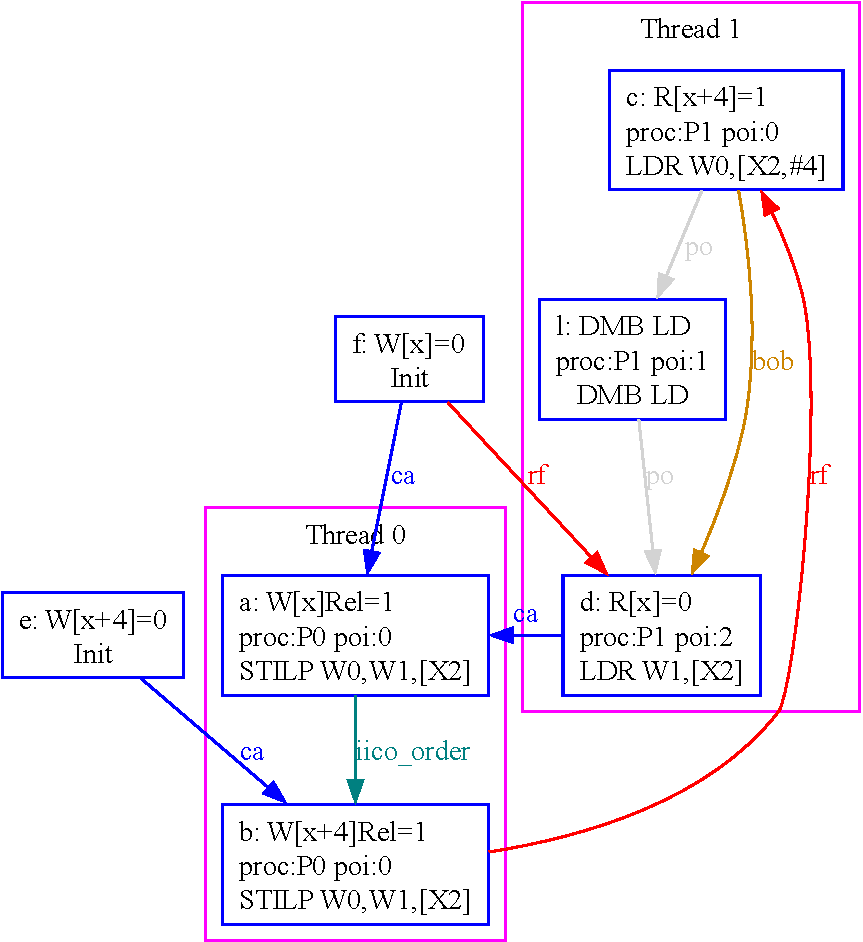
\includegraphics[
    max width=0.8\linewidth
  ]{figures/MP+STILP+dmb.ld-crop.pdf}
  \caption{A candidate execution for \texttt{MP+STILP+dmb.ld}.}
  \label{fig:mp-stilp-dmb-ld-candidate}
\end{figure}

Figure~\ref{fig:mp-stilp-dmb-ld-candidate} shows this graphically.
%
This candidate execution is architecturally Forbidden, due to:
\begin{itemize}
\item The Intrinsic Order Dependency between the Explicit Memory Write Effect
  of x (a) and the Explicit Memory Write Effect of x+4 (b) generated by STILP on P0;
\end{itemize}
combined with:
\begin{itemize}
\item The fact that the Explicit Memory Read Effect
of x+4 (c) generated by the first LDR on P1 Reads-from the
Explicit Memory Write Effect of x (b) generated by
STILP on P0 (represented by b $\xrightarrow{\text{rf}}$ c in the
diagram);
\item The fact that the Explicit Memory Read Effect
of x+4 (c) generated by the first LDR on P1 is Barrier-ordered-before
Explicit Memory Read Effect of x (d) generated by
the second LDR on P0 (represented by c $\xrightarrow{\text{bob}}$ d in the
diagram);
\item The fact that the Explicit Memory Read Effect
of x (d) generated by the second LDR on P1 Reads-from the
initial state, which is itself overwritten by the
Explicit Memory Write Effect of x (a) generated by
STILP on P0, and as a consequence Effect (d) is
Coherence-before Effect (a).
\end{itemize}

These four relations create a cycle in
Ordered-before, and consequently the candidate
execution is architecturally Forbidden. 

\section{Internal visibility requirements \label{sec:internal-visibility-reqs}}

A number of relations, like program order, are not
included by default in Ordered-before. This is the
case of happenstance relations such as Reads-from
between Effects on the same PE and Coherence Order
between Effects on the same PE.
%
However, the architecture still mandates a number of requirements on these
relations, to provide Architecturally valid values. These all require some work
from the hardware, and are therefore hardware requirements.    

Whilst these requirements are not described as cycles, or loops, in
Ordered-before, they are still described as cycles, in a different collection
of relations.

These requirements apply for single-threaded applications as well as
multi-threaded applications. Arm has chosen to keep them separate from
the External visibility requirement and the definition of
Ordered-before, but with the exception of coWR-Exp this is not
a mathematical necessity, simply a presentation choice.

\subsection{Requirement coRW1-Exp}

Consider the litmus test in Figure~\ref{fig:litmus-corw1}.
\litmusinputwithlink[fig:litmus-corw1]{coRW1}

This test asks whether the following candidate
execution is architecturally allowed: 
\begin{itemize}
\item The Explicit Read Effect generated by LDR
W1,[X0] Reads-from the Explicit Write Effect
generated by STR W2,[X0]. 
\end{itemize}

Figure~\ref{fig:cowr1-exp-candidate} shows this graphically.
% Requirement 1 (rewritten)
This candidate execution is architecturally Forbidden. This places a
requirement on the hardware that if the Explicit Memory Read Effect (a) appears
in program order before the Explicit Memory Write Effect (b), then Effect (a)
is not architecturally Allowed to Read-from Effect (b).

\begin{figure}[!htbp]
  \centering
  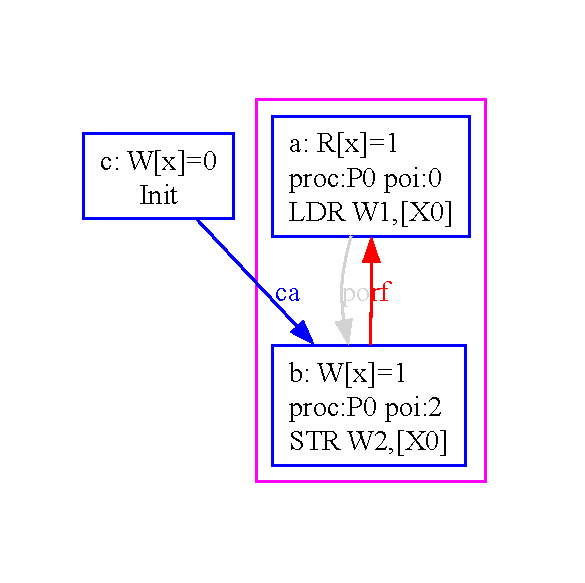
\includegraphics[
    max width=0.4\linewidth
  ]{figures/CoRW1-Exp-crop.pdf}
  \caption{A candidate execution for \texttt{CoRW1-Exp}.}
  \label{fig:cowr1-exp-candidate}
\end{figure}

\subsection{Requirement coWW-Exp}

\litmusinputwithlink[fig:litmus-coww]{coWW}

This test asks whether the following candidate
execution is architecturally allowed:  
\begin{itemize}
\item The Explicit Write Effect generated by STR
W0,[X1] is Coherence-after the Explicit Write Effect
generated by STR W2,[X1]. 
\end{itemize}

Figure~\ref{fig:coww-exp-candidate} shows this graphically.
% Requirement 2 (rewritten)
This candidate execution is architecturally Forbidden. This places a
requirement on the hardware that if the Explicit Memory Write Effect (a)
appears in program order before the Explicit Memory Write Effect (b), then
Effect (a) is not architecturally Allowed to be Coherence-after Effect (b).


\begin{figure}[!htbp]
  \centering
  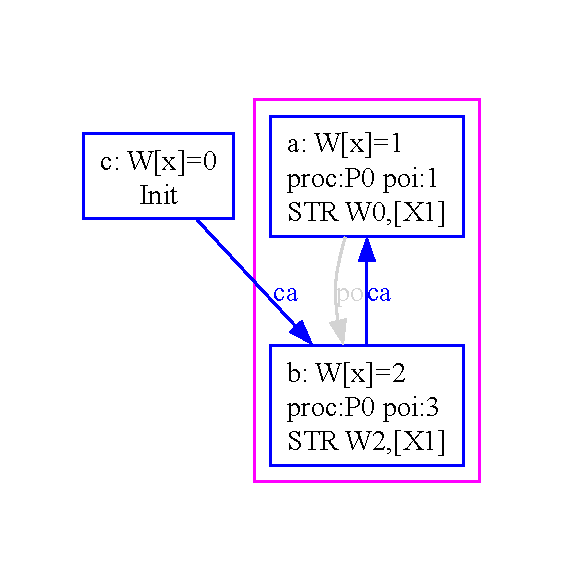
\includegraphics[
    max width=0.4\linewidth
  ]{figures/CoWW-Exp-crop.pdf}
  \caption{A candidate execution for \texttt{CoWW-Exp}.}
  \label{fig:coww-exp-candidate}
\end{figure}

\subsection{Requirement coWR-Exp}
 
\litmusinputwithlink[fig:litmus-cowr]{coWR}

This test asks whether the following candidate
execution is architecturally allowed: 
\begin{itemize}
\item The Explicit Memory Write Effect (a) is
Coherence-after the Memory Write Effect (c) which
corresponds to the inital state 
\item The Explicit Memory Read Effect (b) Reads-from
the Memory Write Effect (c) which corresponds to the
inital state 
\end{itemize}

\begin{figure}[!htbp]
  \centering
  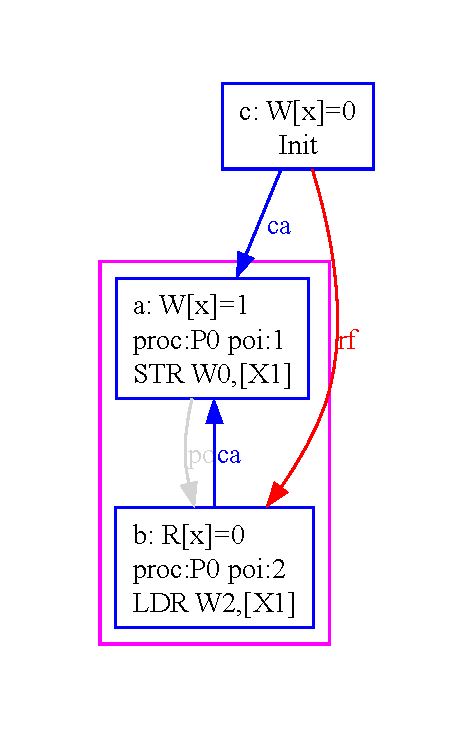
\includegraphics[
    max width=0.3\linewidth,
    max totalheight=0.35\textheight
  ]{figures/CoWR-Exp-crop.pdf}
  \caption{A candidate execution for \texttt{CoWR-Exp}.}
  \label{fig:cowr-exp-candidate}
\end{figure}

Figure~\ref{fig:cowr-exp-candidate} shows this graphically.
% Requirement 3 (rewritten)
This candidate execution is architecturally Forbidden. This places a
requirement on the hardware that if all of the following apply:
\begin{itemize}
  \item the Explicit Memory Write Effect (a) appears in program order before the Explicit Memory Read Effect (b).
  \item Effect (a) is Coherence-after the Memory Write Effect (c).
\end{itemize}
then Effect (b) is not architecturally Allowed to Read-from Effect (c).

Note that this cannot be described as part of Ordered-before, as otherwise we
would be imposing order unduly. Indeed the MP+popl+ctrl-rfi-addr test in
Figure~\ref{fig:litmus-mp-popl-ctrl-rfi-addr} needs to be
Architecturally Allowed (and is readily Observed on deployed hardware), but
would be Forbidden otherwise:

\litmusinputwithlink[fig:litmus-mp-popl-ctrl-rfi-addr]{MP+popl+ctrl-rfi-addr}

\section{\label{sec:external-visibility-reqs} External visibility requirement}

When a relation is included in the overarching Ordered-before relation, it
needs to be in accord with Hardware-requirements. For example, the value a Read
has read cannot be in contradiction with local dependencies on a given PE.

The inclusion of Intrinsic dependencies in
Ordered-before is a requirement: 
\begin{itemize}
\item on the semantics of AArch64 instructions;  
\item on the ordering of Effects generated by the candidate execution of the same AArch64 instruction. 
\end{itemize}

The inclusion of Local hardware requirements in
Ordered-before is a requirement: 
\begin{itemize}
\item on the ordering of Effects generated by different AArch64 instructions;  
\item that the hardware should be able to honour locally, per PE; 
\item without needing to be aware of any Effects generated by another PE. 
\end{itemize}
 
The inclusion of Hazard-ordered-before happenstance
relations in Ordered-before is typically a
requirement:
\begin{itemize}  
\item on the ordering of Memory Read Effects generated by different AArch64 instructions on the same PE; 
\item that the hardware should be able to honour locally, per PE;  
\item but by relying on awareness of Effects generated by other PEs. 
\end{itemize}

The inclusion of other Happenstance relations in
Ordered-before is a requirement: 
\begin{itemize}
\item on the ordering of Memory Effects as they travel through the memory hierarchy, e.g. store buffers and caches; 
\item that the hardware might not be able to honour locally, per PE; 
\item but that might instead require awareness of Effects from multiple PEs that is only known to machinery outside the PE. 
\end{itemize}

\subsection{Local hardware requirements}

Local hardware requirements relations are hardware requirements on the ordering
of Effects which can be honoured locally, per PE.
%
The MP+rel+acq litmus test introduced in
Section~\ref{sec:allowed-memory-effect-interactions} gives examples of Local
hardware requirements relations due to the presence of Store Release
instructions and Load Acquire instructions.
%
These impose requirements on hardware to ensure that the PE honours them. These
requirements can be honoured exclusively within the PE.

\subsection{\label{sec:TLBI-ordered-before} TLBI-ordered-before}

TLBI-ordered-before is a relation at VMSA level that is fundamental to paging.
For example, the litmus test in Figure~\ref{fig:litmus-corr-bbm-w} distils a
Copy-On-Write pattern found in the Linux kernel and thus needs to be Forbidden.
This is a variant of a different litmus test originally contributed by Marc
Zyngier to illustrate the pattern.

\floatinglitmusinputwithlink[fig:litmus-corr-bbm-w]{coRR+BBM+W}

Overall, TLBI-ordered-before formalises situations where there is a message
from one PE to a different PE, and that different PE decides what needs to be
completed in light of that message.
%
For example, in the test in
Figure~\ref{fig:litmus-cowr-tlbi-sync-ishsptev0p}, P0 broadcasts a message to
P1 as part of its execution of the TLB maintenance instruction. Depending on
when P1 receives that message, the Implicit TTD Memory Read Effect E1 generated
by \texttt{STR W3,[X2]} is affected by the TLB invalidation or not.

\begin{itemize}

  \item Executions where the Implicit TTD Memory Read Effect E1 is affected by
    the TLB invalidation but (E1) is also Coherence-before the Explicit Memory
    Write Effect generated by \texttt{STR X1,[X0]} violate the External
    visibility requirement.

  \item Executions where the Implicit TTD Memory Read Effect E1 is not affected
    by the TLB invalidation and the Explicit Memory Read Effect generated by
    \texttt{LDR W4,[X3]} is Coherence-before the Explicit Memory Write Effect
    generated by \texttt{STR W3,[X2]} violate the External visibility
    requirement.

\end{itemize}

So the outcome is Forbidden.

\litmusinputwithlink[fig:litmus-cowr-tlbi-sync-ishsptev0p]{CoWR+tlbi-sync.ishsptev0p}

The definition of TLBI-ordered-before has 3 clauses: the first two are
discussed in this section, and the last one is left for the next section which
pertains to Hazard-ordered-before shapes.

The first clause hinges on a relation called TTD-read-ordered-before, and the
next two clauses extend TTD-read-ordered-before further for cases with other
PEs than the PE issuing the TLBI (this is represented in cat by the use of
the \texttt{ext} construct).

\subsubsection{The general principle of TLBI-ordered-before}

The TLBI-ordered-before relation captures one of the implications of the
synchronization between PEs that may be induced by a TLB maintenance
instruction, i.e. that the TLBI completion waits for concurrent Implicit TTD
Memory Read Effects unaffected by the invalidation.

Each TLB maintenance instruction can be applied to one of the following:
\begin{itemize}
  \item Only the PE that executes the instruction
  \item All PEs in the same Shareability domain as the PE that executes the instruction.
\end{itemize}
The latter applies, for instance, to \texttt{TLBI VAAE1IS} and \texttt{TLBI
VMALLE1IS}, and entails that the PE executing a TLB maintenance instruction
ensures that it completes only after concurrent Implicit TTD Memory Read Effects
in the invalidation scope of the instruction and on PEs in the same Shareability
domain either conclude before the TLB maintenance instruction completes or get
affected by the TLB invalidation.

The TLBI-ordered-before relation provides order from Implicit TTD Memory Read
Effects to Effects known to be ordered after TLBI completes: Effects following a
DSB instruction following the TLBI instruction, or Effects following a DSB and
an ISB instruction following the TLBI instruction. The basis for this ordering
requirement can be illustated using the following diagram.

\begin{center}
\begin{tabular}{l l}
P0                                 &  P1                                        \\
                                   &  Implicit TTD Read E1 (in scope of the TLBI) \\
TLBI Effect E3 $\xrightarrow{\text{sends message}}$ &                                            \\
                                   & $\xleftarrow{\text{sends ack}}$                   \\
                                   &  Implicit TTD Read E2 (in scope of the TLBI)  \\
DSB Full Effect                    &                                            \\
Memory Effect E4                   &                                            \\
\end{tabular}
\end{center}

The PE \texttt{P0} executing a TLB maintenance instruction broadcasts a message
to other PEs in the same Shareability domain as \texttt{P0} (a PE \texttt{P1} on
the diagram), and does not complete the instruction until it receives messages
of acknowledgement from all of them.

PEs receiving the message ensure that outstanding Implicit TTD Memory Read
Effects in the scope of the TLB invalidation result in generating their intended
memory effect, such as an Explicit Memory Effect for a data access or an MMU
Fault. In contrast, Implicit TTD Memory Read Effects that happen after the
message is received are known to be affected by the TLB invalidation. Therefore,
the initiating PE is guaranteed that by the time it receives acknowledgements
from the other PEs, there are no outstanding Implicit TTD Memory Read Effects
not affected by the TLB invalidation.

Concretely, if the message from the TLBI Effect E3 arrives after an Implicit TTD
Memory Read, as is the case for E1 on the diagram, then E1 is considered
TLBI-before E3. If the message from the TLBI Effect E3 arrives before an
Implicit TTD Memory Read, as is the case for E2 on the diagram, then E3 is
considered TLBI-before E2. Note that the point when the message arrives to
\texttt{P1} is arbitrary: there is no assumption in the Concurrency model as to
when this happens, just that for any Implicit TTD Read Effect the TLBI message
is either before or after it. 

The Effect E1 is TTD-read-ordered-before E4 on the diagram, because:
\begin{itemize}
\item E1 is TLBI-before E3, meaning that the TLBI message from E3 arrived to the
PE \texttt{P1} after E1 started, and that E3 waits for E1.
\item E3 is DSB-ordered-before Effect E4 or IFB-ordered-before Effect E4,
meaning that effects ordered by a DSB instruction or a combination of a full DSB
and an ISB instruction end up executing after the full DSB ensures TLBI is
completed.
\end{itemize}
As the first clause of TLBI-ordered-before is exactly TTD-read-ordered-before,
it is also the case that E1 is TLBI-ordered-before E4. In the following
subsections, we illustrate the clauses TLBI-ordered-before with examples.

\subsubsection{First clause of TLBI-ordered-before}

The first clause of TLBI-ordered-before coincides with TTD-read-ordered-before
to capture the idea of TLBIs waiting for Implicit TTD Memory Read Effects.
Consider the following \texttt{MP.V2I+dsb.ish-tlbi.vaae1is-dsh.ish+dsb.ish-isb}
test.

\litmusinputwithlink[fig:litmus-mp-v2i-dsb-ish-tlbi-vaae1is-dsh-ish-dsb-ish-isb]{MP.V2I+dsb.ish-tlbi.vaae1is-dsh.ish+dsb.ish-isb}

In this test, the PTE for a VA~\texttt{x} is initially valid. P0 executes
\texttt{STR X6,[X7]} to make the PTE invalid, and proceeds to executing the
``break'' sequence: a \texttt{DSB ISH}, a \texttt{TLBI VAAE1IS} to the page
holding the VA~\texttt{x} and a \texttt{DSB ISH}. It then sets a flag in memory
by executing \texttt{STR W0,[X1]}.
%
P1 reads the flag from memory by executing \texttt{LDR W0,[X1]}, and executes a
\texttt{DSB ISH} and an \texttt{ISB} barriers, after which it attempts to access
the VA~\texttt{x} by executing \texttt{LDR W2,[X3]}.
%
The question of this test is whether it is possible for P1 to read the updated
value of the flag, but not to raise an MMU Translation Fault upon loading from
the VA~\texttt{x}.

In the executions that could satisfy the exists clause of the test, the Explicit
Memory Write Effect generated by \texttt{STR W0,[X1]} on P0 is read-from by the
Explicit Memory Read Effect generated by \texttt{LDR W0,[X1]} on P1. The
Concurrency model considers two possibilities for how \texttt{TLBI VAAE1IS}
synchronizes with the Implicit TTD Memory Read Effect generated by \texttt{LDR
W2,[X3]}.
\begin{itemize}
\item The first possibility is that the TLBI Effect is TLBI-before the Implicit
TTD Memory Read Effect. When that is the case, the TLBI Effect is
TLBI-coherence-before the Explicit Memory Write Effect generated by \texttt{STR
X6,[X7]} on P0, which in turn is DSB-ordered-before the TLBI Effect. These
relations form a cycle that is in violation of the External Visibility
requirement of the Concurrency model, so such a possibility is not
architecturally allowed.
\item The second possibility is that the Implicit TTD Memory Read Effect is
TLBI-before the TLBI Effect; in this case, the former is also
TLBI-ordered-before the Explicit Memory Write Effect generated by \texttt{STR
W0,[X1]} on P0. Recall that this Explicit Memory Write Effect is read-from by
the Explicit Memory Read Effect generated by \texttt{LDR W0,[X1]} on P1. The
latter is also Instruction-Fetch-Barrier-ordered-before the Implicit TTD Memory
Read Effect generated by \texttt{LDR W2,[X3]} on P1. These relations form a
cycle that is in violation of the External Visibility requirement of the
Concurrency model, so such a possibility is not architecturally allowed.
\end{itemize}

In the executions that could satisfy the exists clause of the test are not
architecturally allowed.

\subsubsection{Second clause of TLBI-ordered-before}

The second clause of TLBI-ordered-before extends TTD-read-ordered-before to
capture the idea of TLBIs waiting for not just Implicit TTD Memory Read Effects,
but also associated Explicit Memory Effects or MMU Faults. Consider the
following \texttt{CoWR+tlbi-sync.ishsptev0p} test:

\litmusinputwithlink[fig:litmus-cowr-tlbi-sync-ishsptev0p-2]{CoWR+tlbi-sync.ishsptev0p}

In this test, the PTE for a VA~\texttt{x} is initially valid. P0 executes
\texttt{STR X1,[X0]} to make the PTE invalid, and proceeds to executing the
``break'' sequence: a \texttt{DSB ISH}, a \texttt{TLBI VAAE1IS} to the page
holding the VA~\texttt{x} and a \texttt{DSB ISH}. It then reads from a
VA~\texttt{z}, which is an alias for VA~\texttt{x}, by executing \texttt{LDR
W4,[X3]}. In parallel, P1 writes 2 into the VA~\texttt{x} by executing
\texttt{STR W3,[X2]}, thus overwriting the initial value of 1.
%
The question of the test is whether at the end of the litmus-test execution it
is possible for the physical address initially corresponding to \texttt{x} to
hold 2, but for the P0 to read 1 via the alias.

In the executions that could satisfy the exists clause of the test, the Explicit
Memory Write Effect generated by \texttt{STR W3,[X2]} on P1 is the final write
to the physical address \texttt{x} is mapped to. The Explicit Memory Read Effect
generated by \texttt{LDR W4,[X3]} on P0 is coherence-before that Explicit
Memory Write Effect.

The Concurrency model considers two possibilities for how \texttt{TLBI VAAE1IS}
synchronizes with the Implicit TTD Memory Read Effect generated by \texttt{STR
W3,[X2]}.
\begin{itemize}
\item The first possibility is that the TLBI Effect is TLBI-before the Implicit
TTD Memory Read Effect. When that is the case, the TLBI Effect is
TLBI-coherence-before the Explicit Memory Write Effect generated by \texttt{STR
X1,[X0]} on P0, which in turn is DSB-ordered-before the TLBI Effect. These
relations form a cycle that is in violation of the External Visibility
requirement of the Concurrency model, so such a possibility is not
architecturally allowed.
\item The second possibility is that the Implicit TTD Memory Read Effect is
TLBI-before the TLBI Effect; in this case, the former is also
TTD-read-ordered-before the Explicit Memory Read Effect generated by
\texttt{LDR W4,[X3]} on P0. The second clause of the TLBI-ordered-before is
that the Explicit Memory Write Effect generated by \texttt{STR W3,[X2]} on P1 is
TLBI-ordered-before the Explicit Memory Read Effect generated by \texttt{LDR
W4,[X3]}. Recall that the latter is coherence-before the former. These
relations form a cycle that is in violation of the External Visibility
requirement of the Concurrency model, so such a possibility is not
architecturally allowed.
\end{itemize}

\subsection{Hazard-ordered-before happenstance relations}

Hazard-ordered-before happenstance relations are  hardware requirements on the
ordering of Effects which can be honoured locally, per PE, but relying on
awareness of Effects generated by other PEs.

All Hazard-ordered-before relations aim to architecturally Forbid a ``triangle'' shape, where:
\begin{itemize}  
\item a PE P0 generates an Effect (a);  
\item a PE P1 generates two Read Effects (b) and (c)
in program order, such that:  
  \begin{itemize}
  \item the first of these two Read Effects (b) observes P0’s Effect (a);
  \item the second of these two Read Effects (c) is ``somehow-ordered-before'' P0’s Effect (a).
  \end{itemize}
\end{itemize}

The architecture mandates that if the second Read
Effect (c) on P1 is ``somehow-ordered-before'' the
Effect (a) on P0, then the first Read Effect (b) on
P1 must not observe the Effect (a) on P0.  
 
Another way of putting it, which might feel less
intuitive to hardware folks, is that these two Read
Effects (b) and (c) require some sort of mechanism to
ensure that the value read by the second Read c is
deemed “architecturally sensible” w.r.t. the first
Read b’s value.  
%
Figure~\ref{fig:hob-candidate} shows this graphically.

\begin{figure}[!htbp]
  \centering
  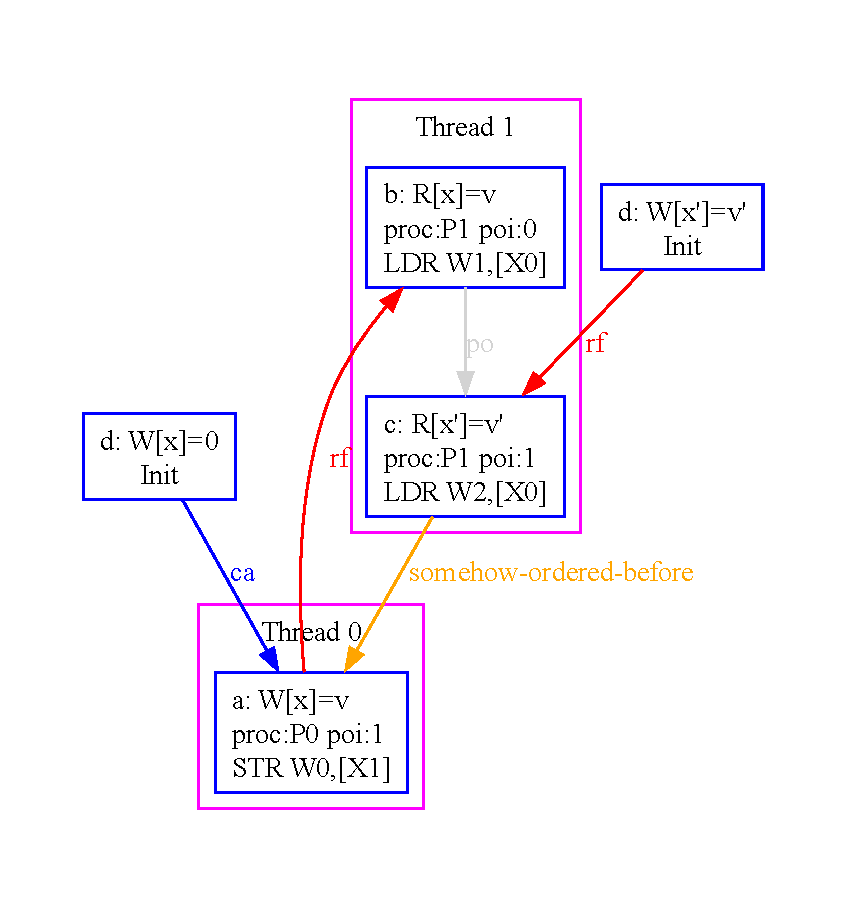
\includegraphics[
    max width=0.55\linewidth
  ]{figures/hob-crop.pdf}
  \caption{A candidate execution for a hazard-ordered-before pattern.}
  \label{fig:hob-candidate}
\end{figure}

In other words, the hardware is required to do some
work to ensure that if the second Read Effect (c) on
P1 is ``somehow-ordered-before'' the Effect (a) on P0,
then it must not be possible for the first Read
Effect (b) on P1 to observe the Effect (a).  
 
The two Reads in program order on P1 can be, for
example:  
\begin{itemize}
\item Explicit Memory Read Effects of the same
Location, which corresponds to the placeholder
``somehow-ordered-before'' relation being replaced by
Coherence-before; 
\item Implicit Translation Table Descriptor Read
Effects, which corresponds to the placeholder
``somehow-ordered-before'' relation being replaced by
TTD-read-ordered-before; 
\item Implicit Instruction Read Effects, which
corresponds to the placeholder
``somehow-ordered-before'' relation being replaced by
Instruction-read-ordered-before.  
\end{itemize}

As a consequence there are currently 3 types of
Hazard-ordered-before happenstance relations, which
correspond to the types of Reads listed above: 
\begin{itemize}
\item Explicit-hazard-ordered-before; 
\item the last aspect of TLBI-ordered-before; 
\item IC-ordered-before. 
\end{itemize} 

In the case of the Reads on P1 being Explicit Memory
Read Effects for example, ``somehow-ordered-before''
means that the value read by R2 is not “older” than
the value read by R1, or in other words, that the
Write from which R2 takes its value does not precede
W in the coherence order.  
 
This requires some work from the hardware, to ensure
that the coherence protocol honours this requirement.
However, in most cases of Hazard-ordered-before, this
work can be done from within the reading PE P1,
provided that the reading PE P1 observes an Effect
from the PE P0, or that the PE P0 sends some sort of
message to facilitate the hazarding.  
 
Note that in the TLBI and IC cases, the hardware
would likely be holding up a barrier preceding the
Effect (a), so that the Effect (a) would not even
happen. By contrast, in the Explicit Reads case, the
Write Effect (a) would be happening, and the hardware
would have to respond to that. 

\subsubsection{Explicit-hazard-ordered-before}

Consider the litmus test in Figure~\ref{fig:litmus-corr}.
\litmusinputwithlink[fig:litmus-corr]{coRR}

This test asks whether the following candidate execution is architecturally allowed: 
\begin{itemize}
\item the Explicit Memory Read Effect generated by LDR W1,[X0] on P1 Reads-from the Explicit Memory Write Effect generated by STR W0,[X1] on P0; 
\item the Explicit Memory Read Effect generated by LDR W2,[X0] on P1 does not read from the Explicit Memory Write Effect generated by STR W0,[X1] on P0, instead taking its value from the initial state. 
\end{itemize}

\begin{figure}[!htbp]
  \centering
  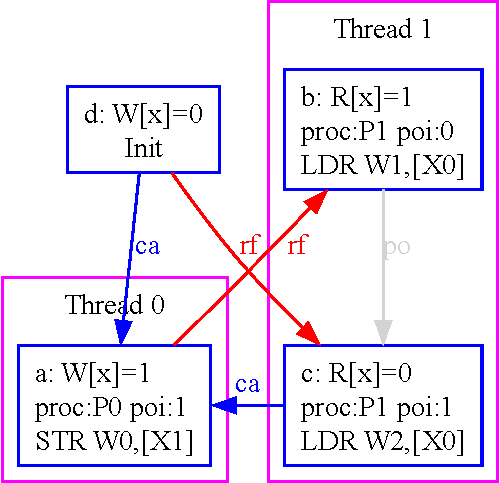
\includegraphics[
    max width=0.5\linewidth,
    max totalheight=0.3\textheight
  ]{figures/CoRR-crop.pdf}
  \caption{A candidate execution for \texttt{CoRR}.}
  \label{fig:corr-candidate}
\end{figure}

Figure~\ref{fig:corr-candidate} shows this graphically.
% Requirement 4 (rewritten)
This candidate execution is architecturally Forbidden. This places a
requirement on the hardware that if all of the following apply:
\begin{itemize}
  \item the Explicit Memory Read Effect (b) appears in program order before the Explicit Memory Read Effect (c).
  \item Effect (c) Reads-from the Memory Write Effect (d).
  \item Effect (d) is Coherence-before the Explicit Memory Write Effect (a).
\end{itemize}
then Effect (b) is not architecturally Allowed to Read-from Effect (a).

A typical way for hardware to build this is as follows: if Effect (c)
Reads-from the initial state (i.e. Effect (d)), then Effect (b) must not
Read-from Effect (a) or an even newer Write Effect in the Coherence order: the
snoop coming across that is relevant is ``a vs c'' (not ``a vs b'').  
 
Another way of putting it, perhaps less intuitive to hardware folks, is that if
the Explicit Memory Read Effect (b) generated by LDR W1,[X0] on P1 Reads-from
the Explicit Memory Write Effect (a) generated by STR W0,[X1] on P0, then the
Explicit Memory Read Effect (c) generated by LDR W2,[X0] on P1 must not read
from an earlier write than a in the Coherence Order.  

Forbidding the behaviour is not inherent to all hardware designs: indeed Sparc
RMO, Alpha, Itanium and IBM PowerPC before Power4 all used to allow the CoRR
behaviour.  This means that this requirement does not fall out naturally, and
requires some work to ensure that the coherence protocol honours it. 
 
In most cases, this work can be done exclusively within the PE P1 using a
signal (e.g. snoop request) sent by the system to PE P1 in response to the
Write Effect (a). PE P1 is able to use this signal to create hazarding between
the two LDRs b and c. The hazarding would need to take some microarchitectural
action (e.g. flush or replay) if the hazarding determined that the second LDR c
provided data from before the signal being received and the first LDR b
provided data from after the signal being received.  
  
In some cases, the PE will not receive a signal from the system in response to
the Write Effect (a). The most notable case of this is when the Location is
non-cacheable. In this case, PE P1 would need to ensure that the two LDRs were
presented to the system interconnect in the correct order and with the correct
attributes (per the interconnect protocol) such that the system machinery
ensures that the architecturally required behavior is not violated. 

\subsubsection{TLBI-ordered-before: hazarding clause}

We reiterate and emphasise that this is only one of the 3 aspects of
TLBI-ordered-before. The other 2 aspects of TLBI-ordered-before are discussed
in Section~\ref{sec:TLBI-ordered-before}.

Consider the litmus test in Figure~\ref{fig:litmus-corr-pte9-mod}.
\litmusinputwithlink[fig:litmus-corr-pte9-mod]{coRR-pte9-mod}

This test asks whether the following candidate execution is architecturally allowed: 
\begin{itemize}
\item the Implicit TTD Read of PTE(x) generated by LDR W2,[X1] on P1 Reads-from the Explicit Memory Write of PTE(x) generated by STR X4,[X3] on P0; 
\item the Implicit TTD Memory Read Effect of TTD(x) generated by LDR W4,[X1] on P1 takes its value from the initial state. 
\end{itemize}

\begin{figure}[!htbp]
  \centering
  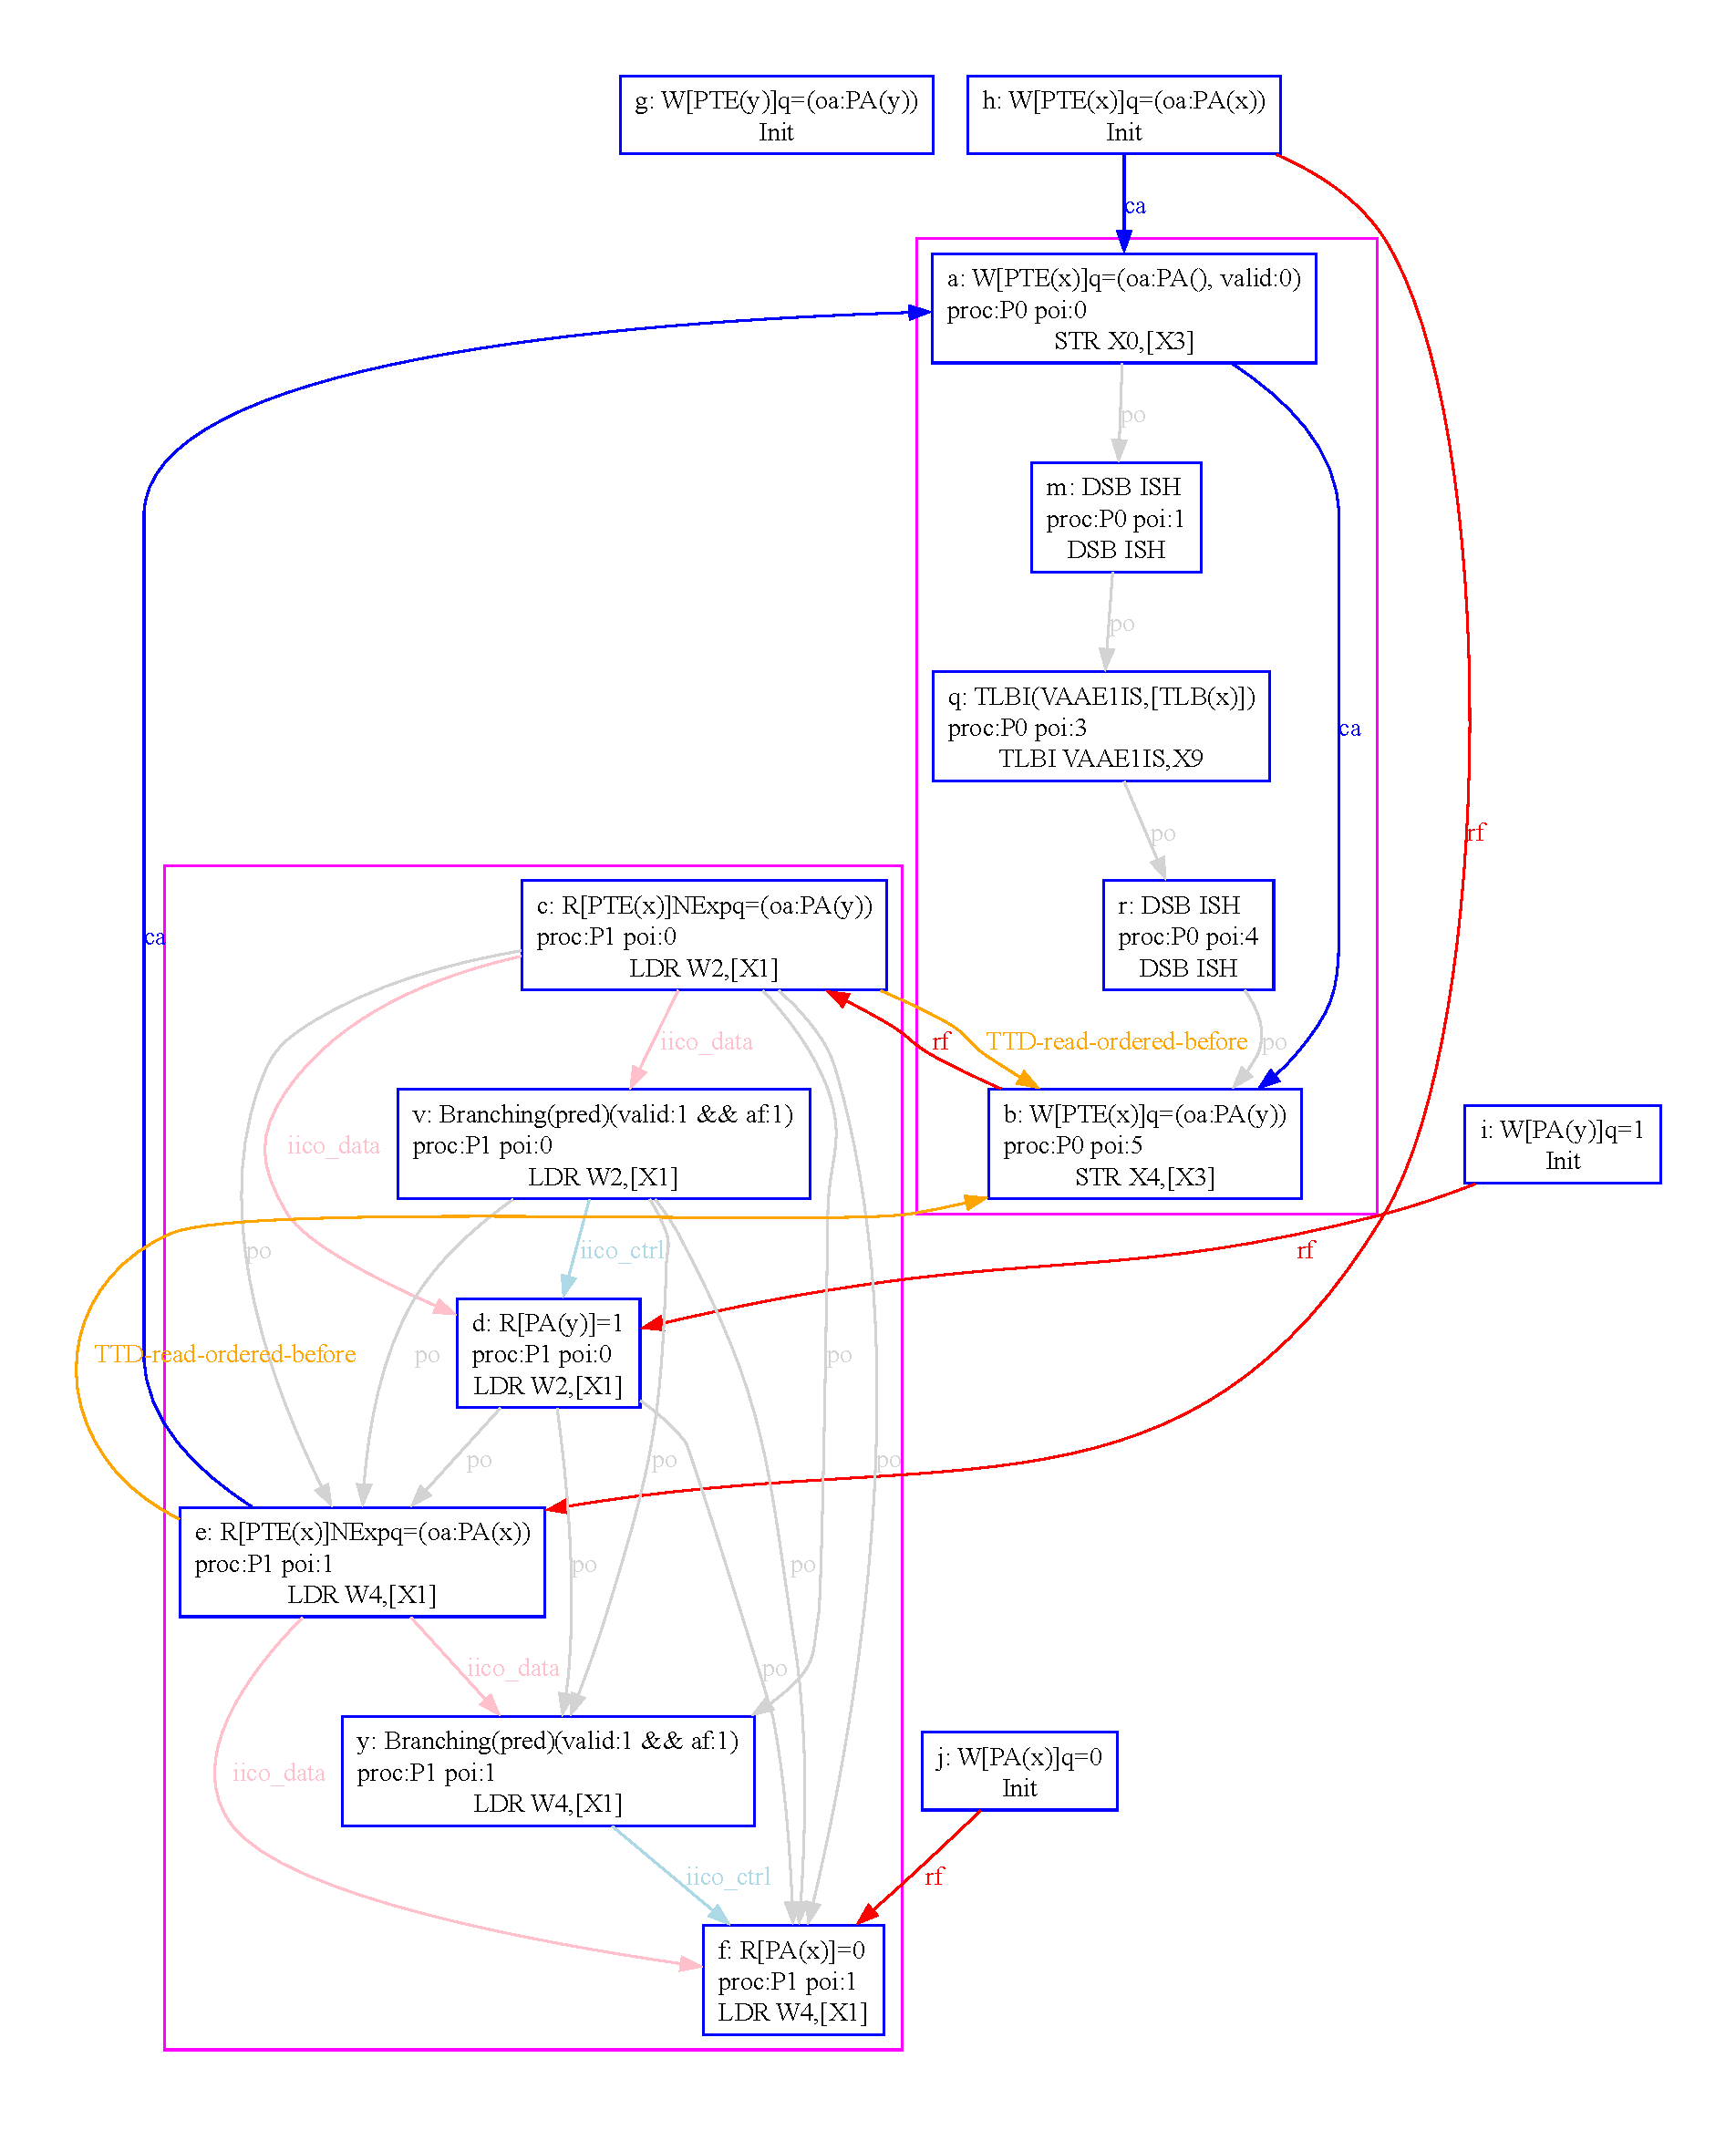
\includegraphics[
    max width=\linewidth
  ]{figures/coRR-pte9-mod-00-2.dot-crop.pdf}
  \caption{A candidate execution for \texttt{coRR-pte9-mod}.}
  \label{fig:corr-pte9-mod-candidate}
\end{figure}

Figure~\ref{fig:corr-pte9-mod-candidate} shows this candidate
execution graphically.
% Requirement 5 (rewritten)
This candidate execution is architecturally Forbidden.
%
This places a requirement on the hardware that if all of the following apply:
\begin{itemize}
  \item the Implicit TTD Memory Read Effect (c) is Translation-intrinsically-before the Explicit Memory Read Effect (d).
  \item Effect (d) and the Explicit Memory Read Effect (f) have the Same Low-order Bits.
  \item Effect (d) appears in program order before Effect (f).
  \item the Implicit TTD Memory Read Effect (e) is Translation-intrinsically-before Effect (f).
  \item Effect (e) and Effect (c) are generated in the same translation context.
  \item Effect (e) is TLBI-before the TLBI Effect (q).
  \item the DSB FULL Effect (r) appears in program order between Effect (q) and the Explicit Memory Write Effect (b).
\end{itemize}
then the hardware is not architecturally Allowed to let Effect (c) Read-from Effect (b).
%
More precisely, if Effect (e) is in scope of the TLBI Effect (q) on P0, then
Effect (c) will be Ordered-before Effect (b), and as a consequence Effect (c)
cannot Read-from Effect (b). 
 
Another way of putting it, which might feel less intuitive to hardware folks,
is that if the Implicit TTD Memory Read Effect (c) generated by LDR W2,[X1] on
P1 Reads-from the Explicit Memory Write Effect (b) generated by STR X4,[X3] on
P0, then the Implicit TTD Memory Read Effect (e) generated by LDR W4,[X1] on P1
must not be Ordered-before the Explicit Memory Write Effect (b).  

This is depicted by the arrow labelled TTD-read-ordered-before in the diagram above. As the Implicit TTD Memory Read Effect (c) and the Implicit TTD Memory Read Effect (e) are to virtual addresses with the same low-order bits (in fact, the same virtual address in this case), by definition of TLBI-ordered-before, the Implicit TTD Memory Read Effect (c) is TLBI-ordered-before the Explicit Memory Write Effect (b). 

Forbidding the behaviour is achieved through considering the ordering implications of concurrent TLB maintenance sequences. 
 
This work can be done exclusively within the PE P1, provided that some signal (e.g. a DVM message due to a concurrent TLBI Effect) is sent by P0. Intuitively, this can be understood through considering two possibilities: whether the message due to the TLBI Effect (q) is ordered before or after the Implicit TTD Memory Read Effect (e). 
 
When the message due to the TLBI Effect (q) is ordered before the Implicit TTD Memory Read Effect (e), the Explicit Memory Write Effect (a) is visible to the Implicit TTD Memory Read Effect (e). The TLBI-coherence-after ordering rule forbids the latter not to read from the more recent write than the initialization. 
 
When the message due to the TLBI Effect (q) is ordered after the Implicit TTD Memory Read Effect (e) as depicted on the candidate execution graph above (meaning that the corresponding Explicit Memory Effect (f) completed before the TLBI completed), the Implicit TTD Memory Read Effect (e) is Ordered-before the Explicit Memory Write Effect (b), since latter follows the completed TLBI. Furthermore, Effect (c) is also architecturally required to be Ordered-before Effect (b) in this case. 

\subsubsection{IC-ordered-before (when DIC=0)}

The Arm architecture requires the hardware to ensure coherency between instruction caches and data caches with the help of explicit use of data cache clean and instruction cache invalidation when the DIC and IDC bits of the CTR\_EL0 register are 0. Practically, this means that the cache maintenance sequence with DC CVAU and IC IVAU is needed to ensure coherence between Explicit Write Memory Effects and Implicit Instruction Read Memory Effects. 
 
Consider the litmus test in Figure~\ref{fig:litmus-mp-ff-dc-cvau-dsb-ish-ic-ivau-dsb-ish-po}.
\litmusinputwithlink[fig:litmus-mp-ff-dc-cvau-dsb-ish-ic-ivau-dsb-ish-po]{MP.FF+dc.cvau-dsb.ish-ic.ivau-dsb.ish+po}
 
This test asks whether the following candidate
execution is architecturally allowed: 
\begin{itemize}
\item the Implicit Instruction Fetch Read generated
by NOP on P1 Reads-from the Explicit Memory Write
Effect generated by STR W2,[X4] on P0; 
\item the Implicit Instruction Fetch Read generated
by m1: B end on P1 takes its value from the initial
state. 
\end{itemize} 

\begin{figure}[!htbp]
  \centering
  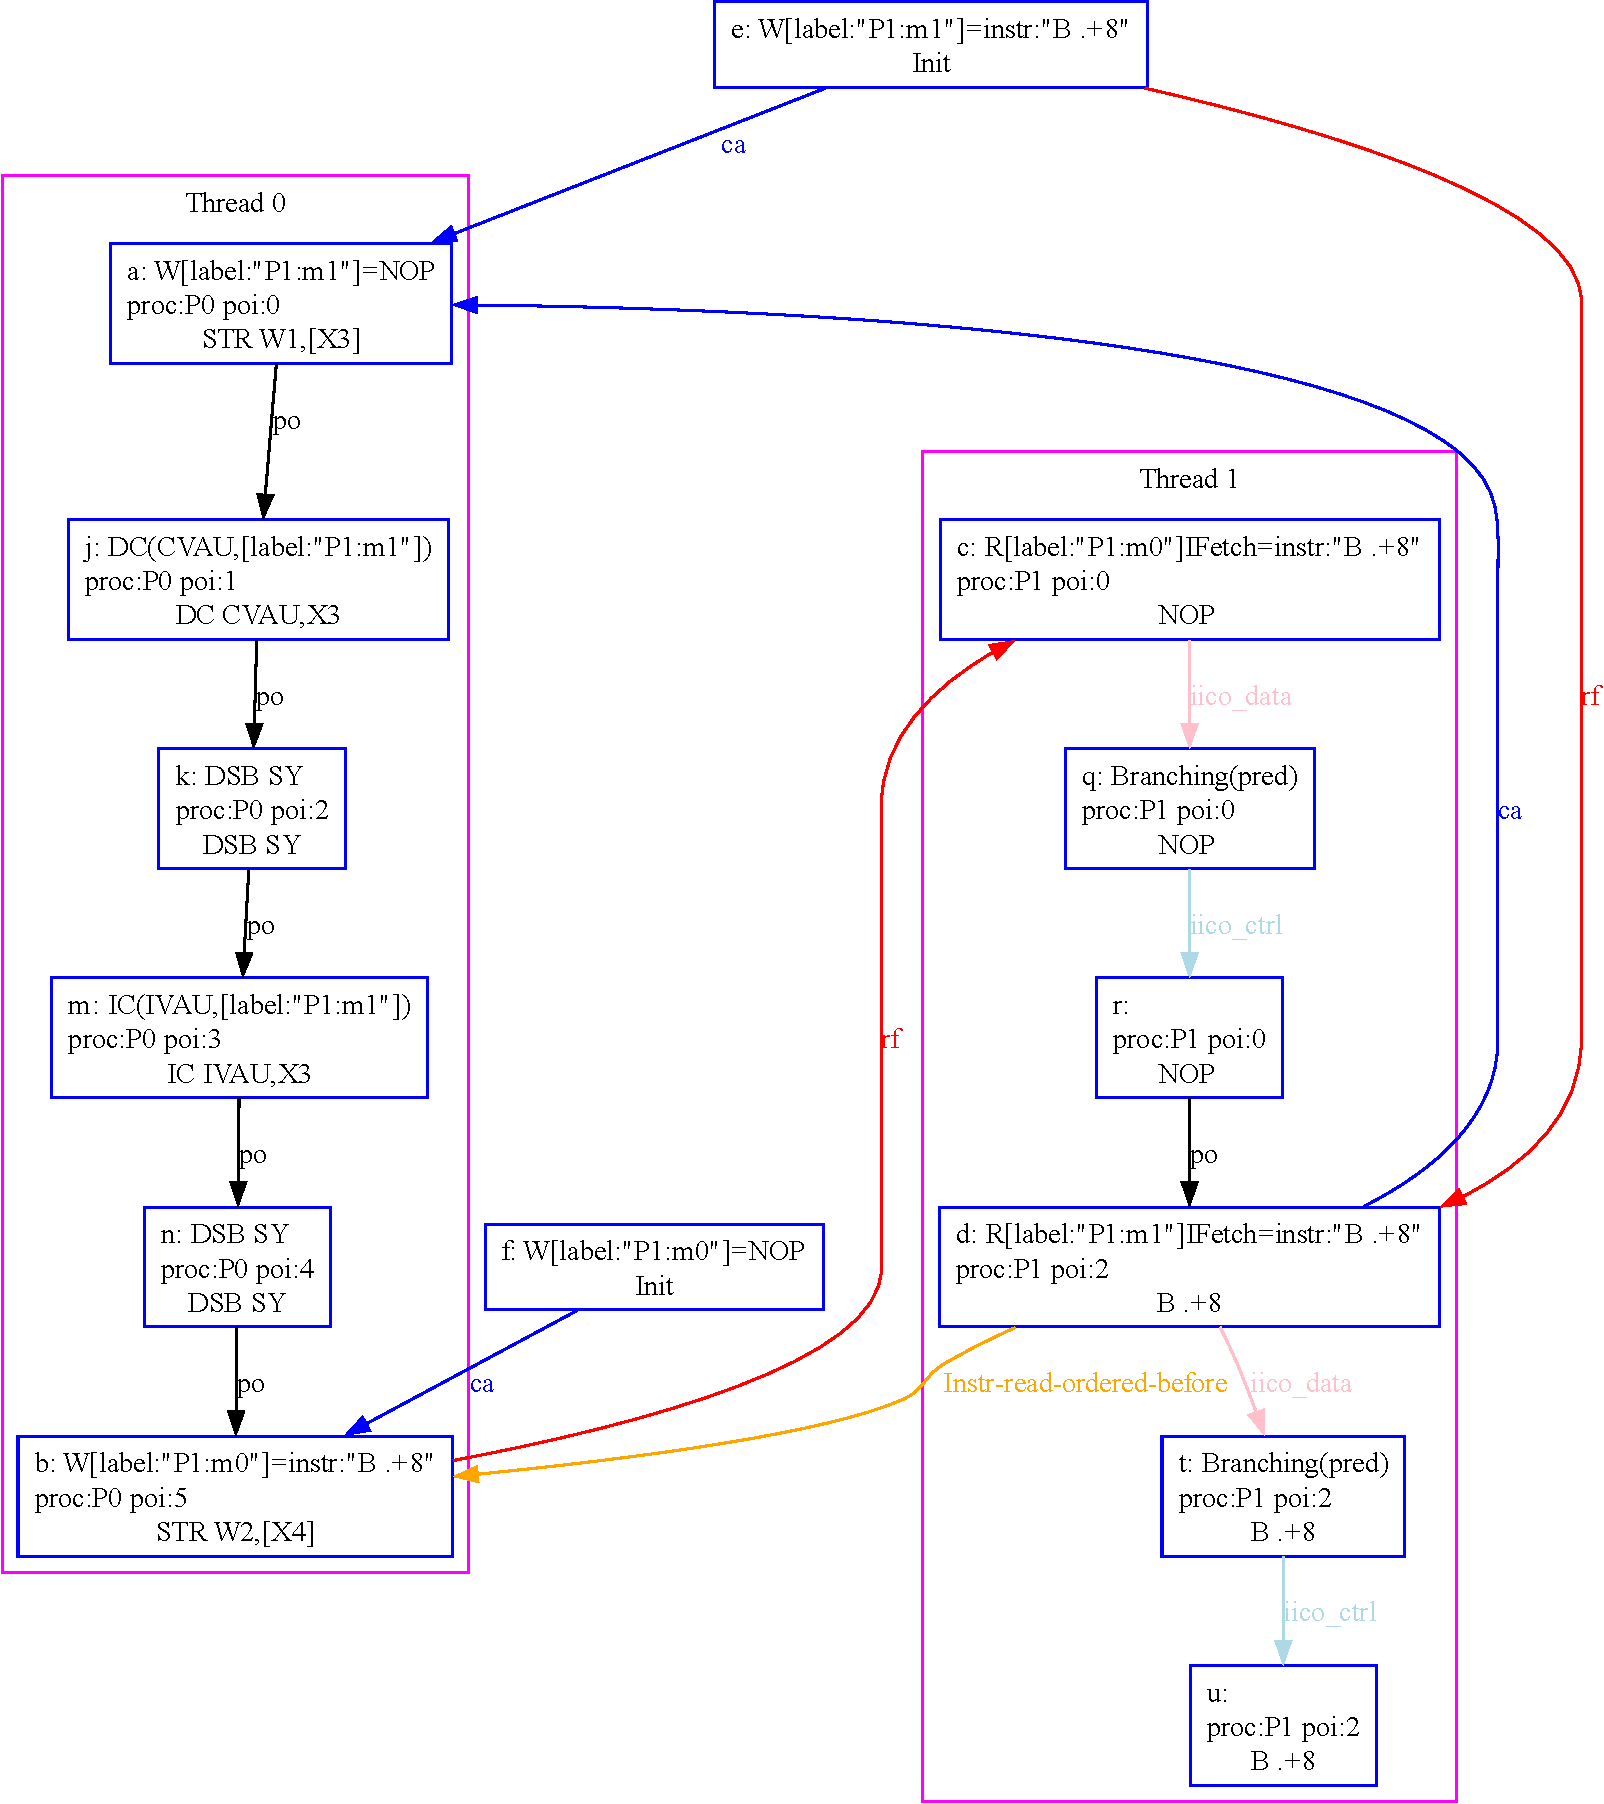
\includegraphics[
    max width=\linewidth
  ]{figures/MP.FF+dc.cvau-dsb.ish-ic.ivau-dsb.ish+po.dot-crop.pdf}
  \caption{A candidate execution for
    \protect\path{MP.FF+dc.cvau-dsb.ish-ic.ivau-dsb.ish+po}.}
  \label{fig:mp-ff-cache-maint-candidate}
\end{figure}

Figure~\ref{fig:mp-ff-cache-maint-candidate} shows this candidate
execution graphically.
% Requirement 6 (rewritten)
This candidate execution is architecturally Forbidden. This places a
requirement on the hardware that if all of the following apply:
\begin{itemize}
  \item the Implicit Instruction Memory Read Effect (c) appears in program order before the Implicit Instruction Memory Read Effect (d).
  \item Effect (d) is IC-before the IC Effect (m).
  \item the DSB FULL Effect (n) appears in program order between Effect (m) and the Explicit Memory Write Effect (b).
\end{itemize}
then Effect (c) is not architecturally Allowed to Read-from Effect (b).
%
More precisely, if DIC=0: if Effect (d) is in scope of the IC Effect (m), then
Effec (d) is Ordered-before Effect (b) and as a consequence Effect (c) on P1
must not Read-from the Effect (b) on P0 or an Effect that is Coherence-after
Effect (b).

Another way of putting it, which might feel less intuitive to hardware folks, is that if the Implicit Instruction Fetch Read c generated by NOP on P1 reads from the Explicit Memory Write Effect (b) generated by STR W2,[X4] on P0, then the Implicit Instruction Fetch Read Effect (d) generated by m1: B end on P1 must NOT be Ordered-before the Explicit Memory Write Effect (b). This is depicted by the arrow labelled Inst-read-ordered-before in the diagram above.  
 
Forbidding the behaviour is not inherent to all hardware designs: this requirement 
requires some work to ensure that the instruction cache protocol honours it. 
 
This work can be done exclusively within the PE P1 – provided that some signal (e.g.  a message due to a concurrent IC IVAU Effect) is sent by P0. Intuitively, this can be understood through considering two possibilities: whether the message due to the IC IVAU Effect (m) happens to be before or after the Implicit Instruction Memory Read Effect (d). 

When the message due to the IC IVAU Effect (m) happens to be before the Implicit Instruction Memory Read Effect (d), the Explicit Memory Write Effect (a) and the subsequent DC CVAU Effect (j) are visible to the Implicit Instruction Memory Read Effect (d). The IC-coherence-after ordering rule forbids the latter not to Read-from the most recent Write Effect. 
 
When the message due to the IC IVAU Effect (m) is happens to be after the Implicit Instruction Memory Read Effect (d) as depicted on the candidate execution graph above (meaning that the corresponding memory accesses completed before the IC completed), the Implicit Instruction Memory Read Effect d is Ordered-before the Explicit Memory Write Effect (b), since latter follows the completed IC IVAU.  Furthermore, Effect (c) is also architecturally required to be Ordered-before Effect (b) in this case. 

\subsubsection{IC-ordered-before (when DIC=1)}

The Arm architecture requires the hardware to ensure coherency between instruction caches and data caches for completed writes when the DIC bit of the CTR\_EL0 register  is 1. Practically, this means that the cache maintenance sequence with DC CVAU and IC IVAU is not needed to ensure coherence between Explicit Write Memory Effects and Implicit Instruction Read Memory Effects. 
 
Consider the litmus test in Figure~\ref{fig:litmus-dic1-mp-ff-dmb-st-po}.

\litmusinputwithlink[fig:litmus-dic1-mp-ff-dmb-st-po]{DIC1.MP.FF+dmb.st+po}

This test asks whether the following candidate execution is architecturally allowed: 
\begin{itemize}
\item the Implicit Instruction Fetch Read Effect at label m0 on P1 Reads-from the Explicit Memory Write Effect generated by STR W2,[X4] on P0; 
\item the Implicit Instruction Fetch Read Effect at label m1 on P1 takes its value from the initial state. 
\end{itemize} 

\begin{figure}[!htbp]
  \centering
  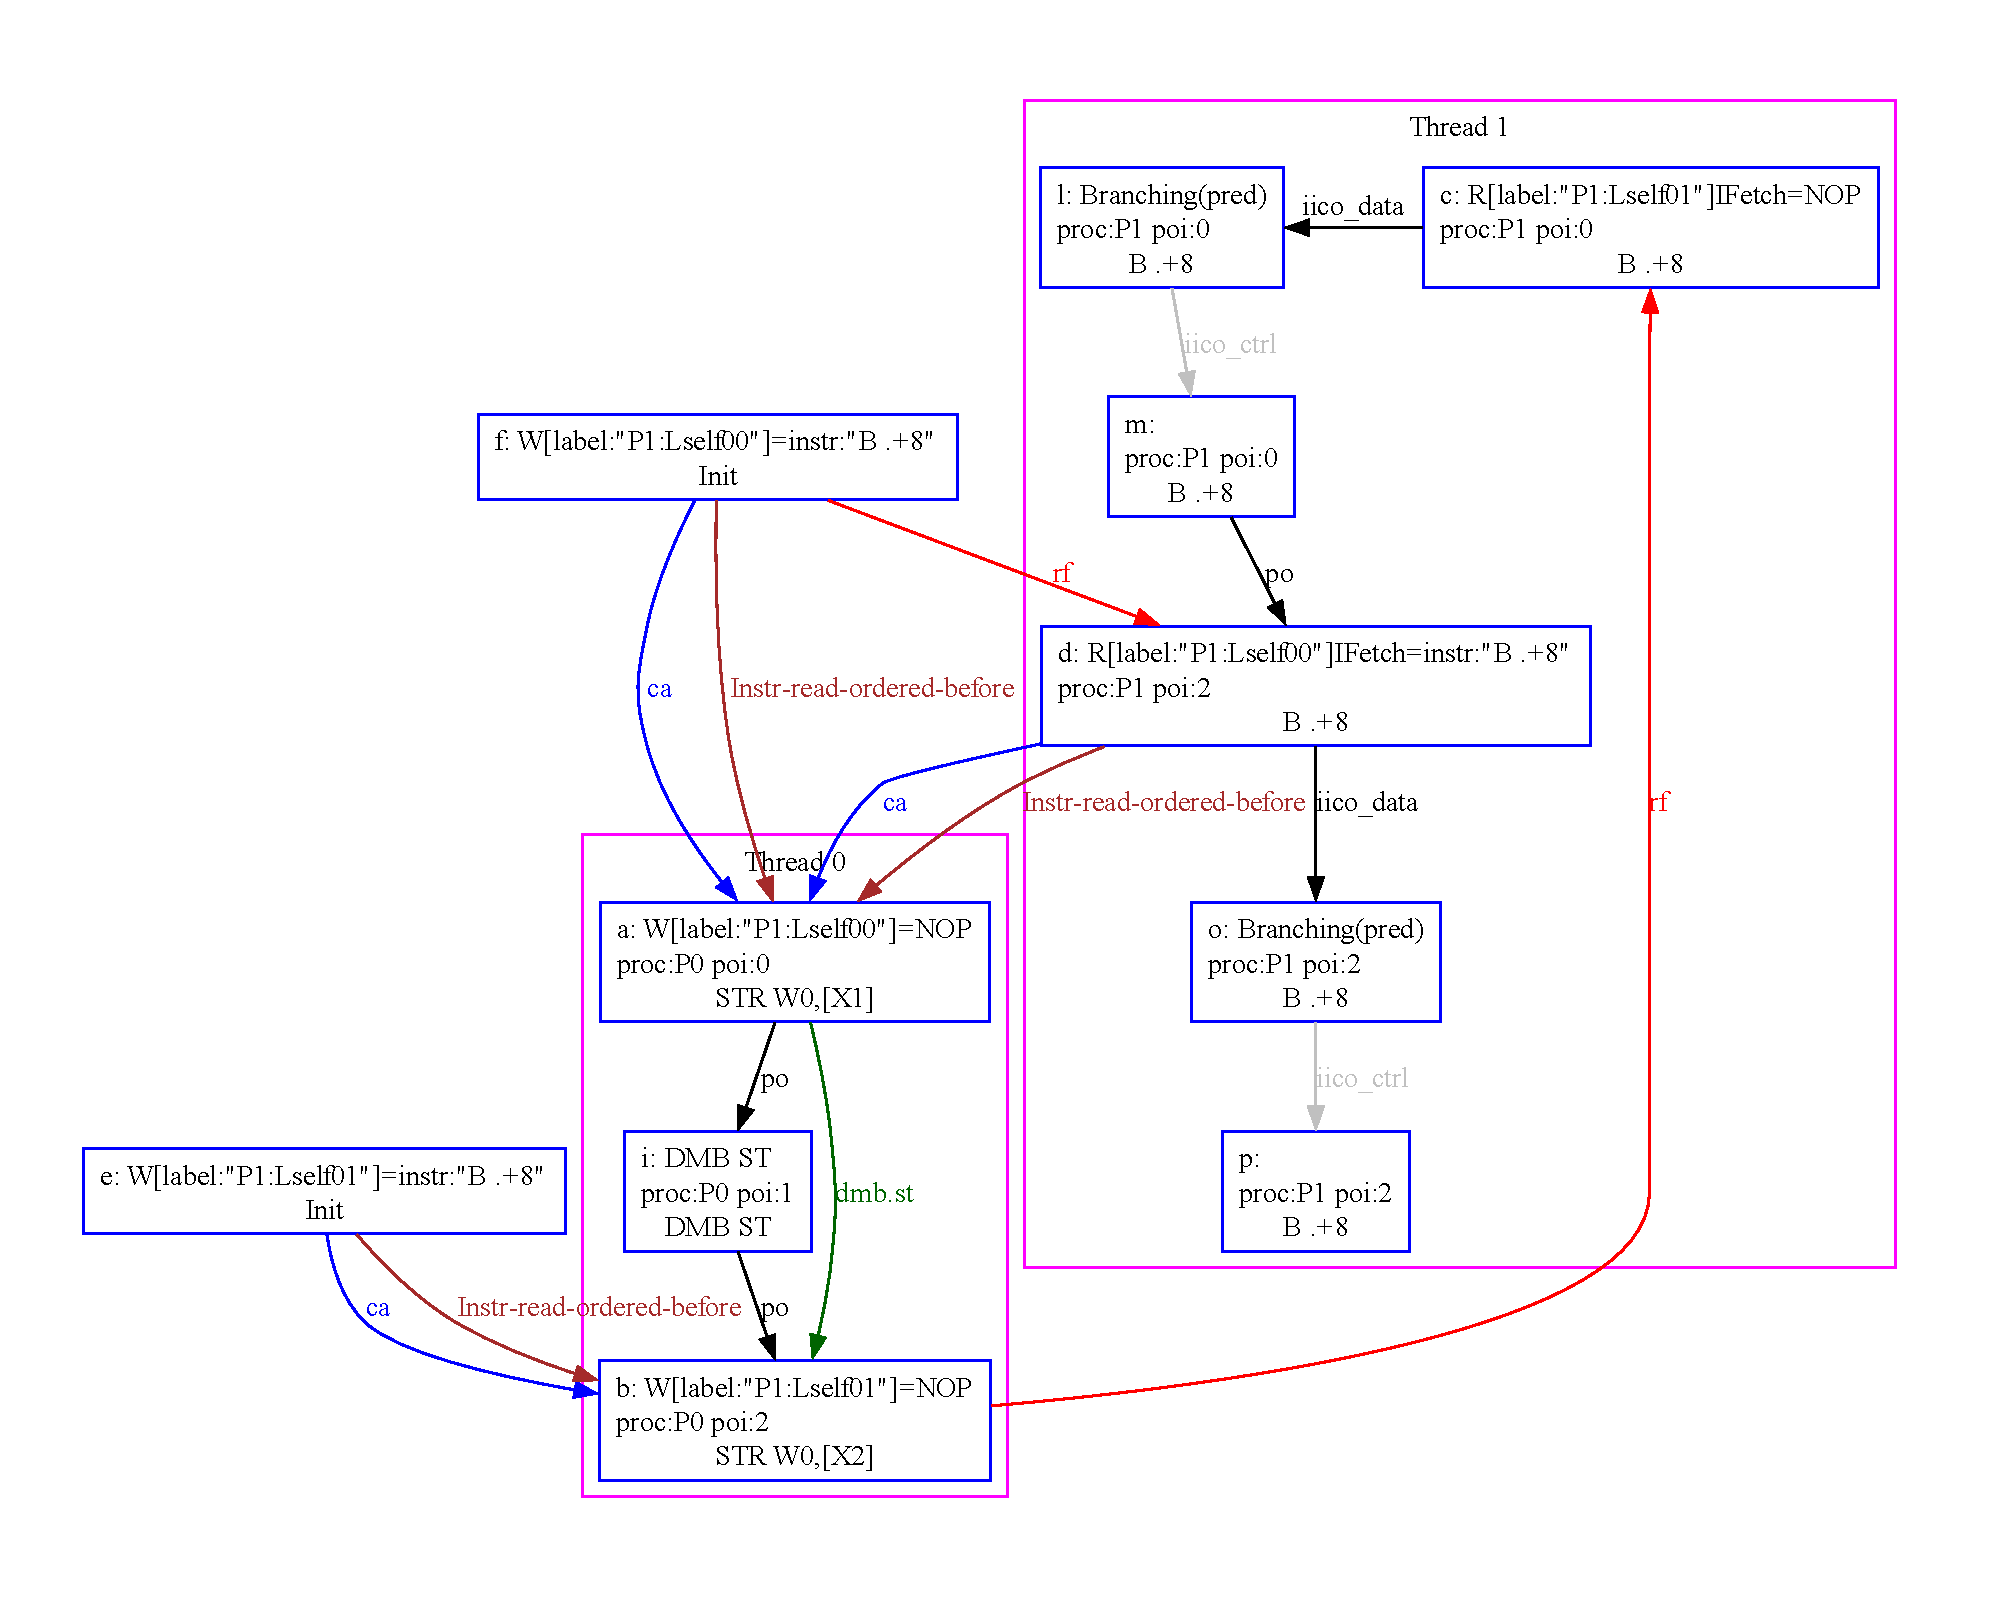
\includegraphics[
    max width=\linewidth
  ]{figures/DIC1.MP.FF+dmb.st+po.dot-crop.pdf}
  \caption{A candidate execution for \texttt{DIC1.MP.FF+dmb.st+po}.}
  \label{fig:dic1-mp-ff-dmb-st-candidate}
\end{figure}

Figure~\ref{fig:dic1-mp-ff-dmb-st-candidate} shows this candidate
execution graphically.
% Requirement 6.5 (rewritten)
This candidate execution is architecturally Forbidden when DIC=1.
%
This places a requirement on the hardware that if all of the following apply:
\begin{itemize}
  \item the Implicit Instruction Memory Read Effect (d) is Ordered-before
    the Explicit Memory Write Effect (b) (given that Effect (d) is
    Instruction-read-ordered-before the Explicit Memory Write Effect (a),
    and the DMB ST Effect (i) appears in program order between Effect (a) and Effect (b)).
  \item the Implicit Instruction Memory Read Effect (c) appears in program order before Effect (d).
\end{itemize}
then Effect (c) is not architecturally Allowed to Read-from Effect (b).
%
More precisely, when DIC=1, if Effect (d) Reads-from an Effect that is
Coherence-before Effect (a), then Effect (c) must not Read-from Effect (b) or
an Effect that is Coherence-after Effect (b).  

Another way of putting it, which might feel less intuitive to hardware folks, is that if the Implicit Instruction Fetch Read Effect (c) generated by NOP on P1 Reads-from the Explicit Memory Write Effect (b) generated by STR W2,[X4] on P0, then the Implicit Instruction Fetch Read Effect (d) generated by m1: B end on P1 must NOT be Ordered-before the Explicit Memory Write Effect (a). This is depicted by the arrow labelled Inst-read-ordered-before in the diagram above.  

\subsection{Other happenstance relations}

Other happenstance relations, when included in Ordered-before, are hardware
requirements that might require awareness of Effects from multiple PEs that is
only known to machinery outside the PE.

Consider the litmus test in Figure~\ref{fig:litmus-sb-rfi-dmb-ld-rfi-dmb-ld}.
\litmusinputwithlink[fig:litmus-sb-rfi-dmb-ld-rfi-dmb-ld]{SB+rfi-dmb.ld+rfi-dmb.ld}

This test asks whether the following candidate execution is architecturally allowed: 
\begin{itemize}
\item the Explicit Memory Read Effect generated by LDR W2,[X1] on P0 (resp. LDR W2, [X3] on P1) Reads-from the Explicit Memory Write Effect generated by STR W0,[X1] on P0 (resp. STR W0,[X3] on P1); 
\item the Explicit Memory Read Effect generated by LDR W4,[X3] on P0 (resp. LDR W4, [X1] on P1) Reads-from the Explicit Memory Write Effect generated by STR W0,[X3] on P1 (resp. STR W0, [X1] on P0). 
\end{itemize} 

\begin{figure}[!htbp]
  \centering
  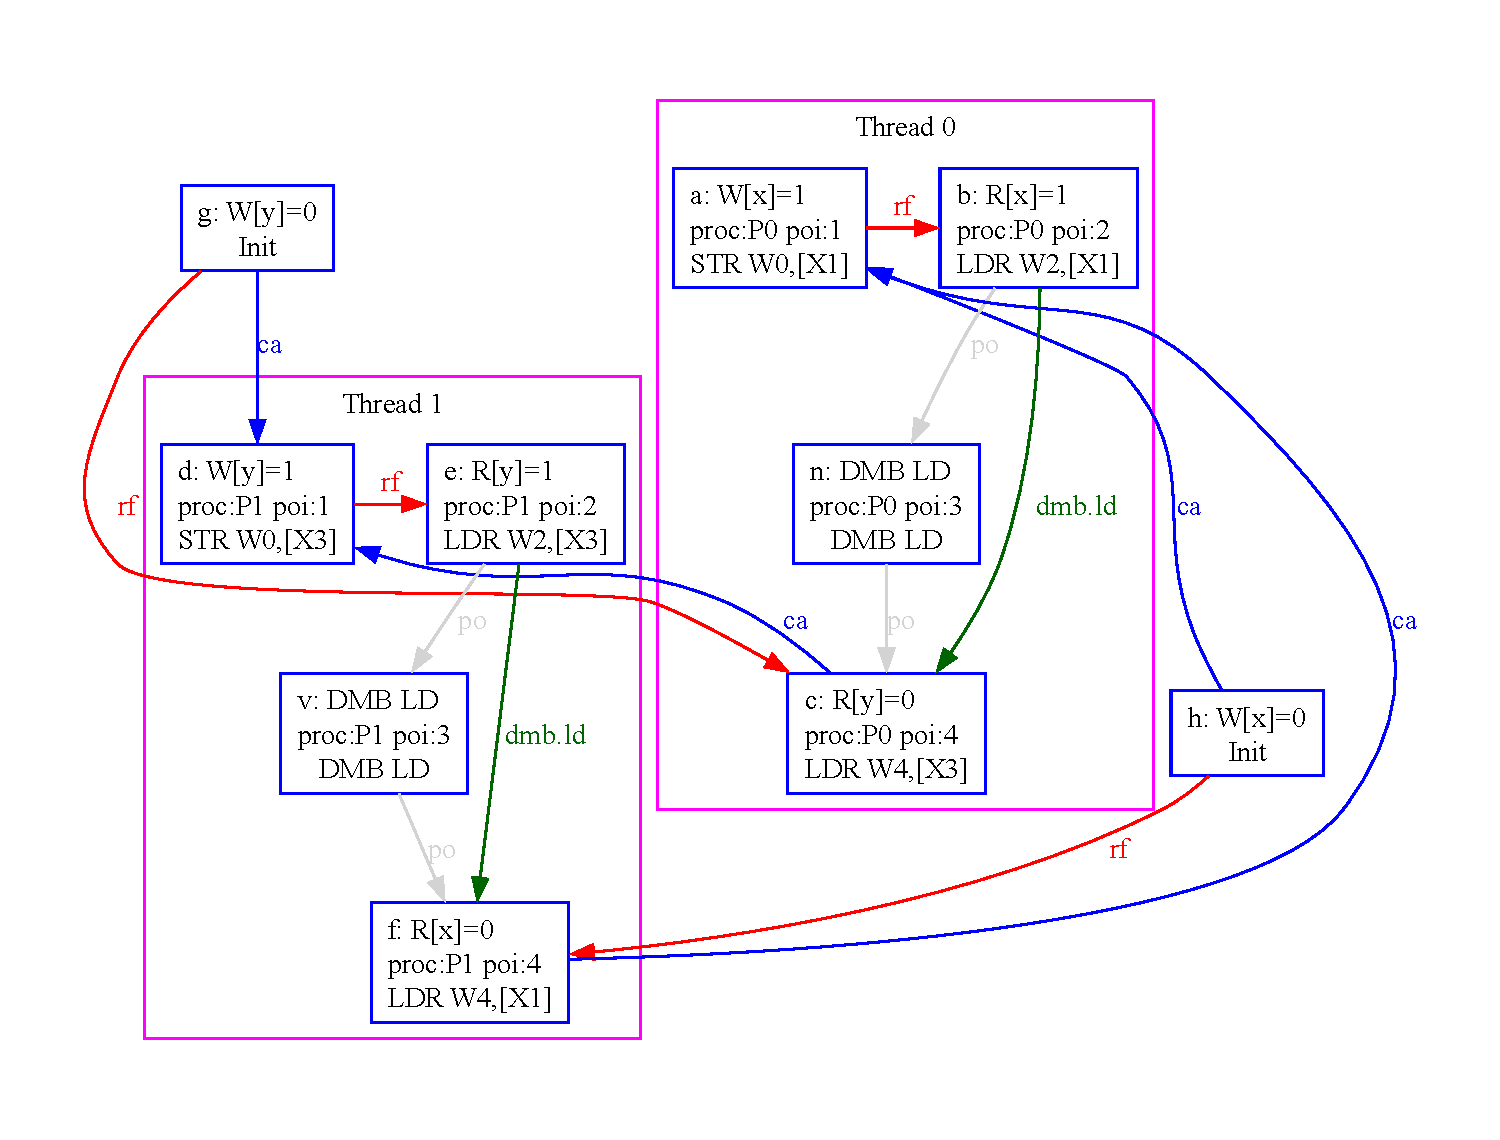
\includegraphics[
    max width=\linewidth
  ]{figures/SB+rfi-dmb.ld+rfi-dmb.ld.dot-crop.pdf}
  \caption{A candidate execution for \texttt{SB+rfi-dmb.ld+rfi-dmb.ld}.}
  \label{fig:sb-rfi-dmb-ld-candidate}
\end{figure}

Figure~\ref{fig:sb-rfi-dmb-ld-candidate} shows this candidate
execution graphically.
%
This candidate execution is architecturally Allowed. In other words, the Arm Concurrency Model does not place a requirement on hardware to provide order from the Explicit Memory Write Effect (a) of the STR W0,[X1] on P0 (resp. STR W0,[X3] on P1) to the Explicit Memory Read Effect (b) of the LDR W2,[X1] on P0 (resp. LDR W2,[X3] on P1). 
 
This enables the use of store buffers in hardware designs, more precisely it permits a load (e.g. LDR W2,[X1] on P0) to take a value from a store buffer “early”, or at least earlier than other PEs: the Explicit Memory Read Effect (b) generated by the LDR W2,[X1] on P0 can read from the Explicit Memory Write Effect (a) generated by the STR W0,[X1] on P0, and this well before the value becomes visible to the LDR W4,[X1] on P1.  
 
On the contrary, consider the case where the store instructions are moved to different PEs, as in the IRIW+dmb.lds example in Figure~\ref{fig:litmus-iriw-dmb-lds}.
\litmusinputwithlink[fig:litmus-iriw-dmb-lds]{IRIW+dmb.lds}

In this situation, the corresponding candidate execution shown in
Figure~\ref{fig:iriw-dmb-lds-candidate} becomes architecturally Forbidden.

\begin{figure}[!htbp]
  \centering
  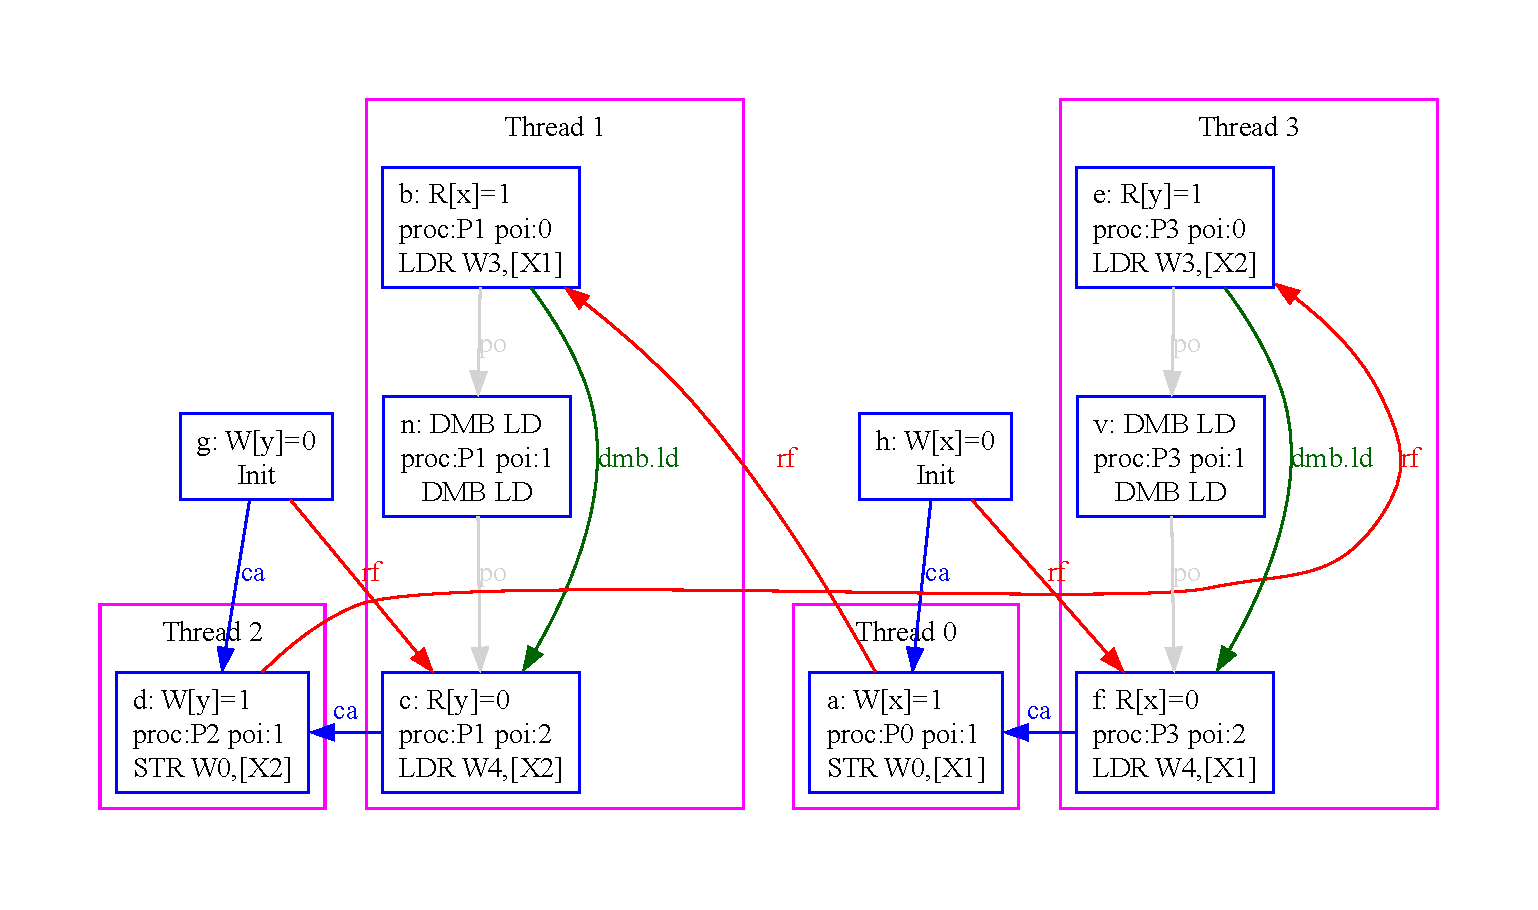
\includegraphics[
    max width=\linewidth
  ]{figures/IRIW+dmb.lds.dot-crop.pdf}
  \caption{A candidate execution for \texttt{IRIW+dmb.lds}.}
  \label{fig:iriw-dmb-lds-candidate}
\end{figure}

% Requirement 9 (rewritten)
This places a requirement on the hardware that if all of the following apply:
\begin{itemize}
  \item the Memory Read Effect (b) Reads-from the Memory Write Effect (a).
  \item the Memory Read Effect (f) and Effect (b) are to the same location.
  \item Effect (f) is Ordered-after Effect (b).
  \item the Memory Write Effect (h) is Coherence-before Effect (a).
\end{itemize}
then Effect (f) is not architecturally Allowed to Read-from Effect (h).
%
More generally, if by happenstance Effect (b) Reads-from Effect (a), then all
Read Effects which have the same Location as (b) and are Ordered-after (b) must
Read-from Effect (a) or an Effect later than (a) in Coherence order, ensuring
that nothing thereafter can observe any Effect before (a).

This requirement prohibits certain hardware designs which would be permitted by IBM PowerPC.
About a decade ago, this requirement was thought to hinder scalability but the stance has now changed---indeed Arm has now enshrined this requirement in its Concurrency Model, by making the Concurrency Model “Other-Multi-Copy-Atomic”. 
 
In turn this requirement permits the implementation of barriers which are much more lightweight than IBM PowerPC’s sync barrier: there is no need to implement a barrier which sends a signal to all PEs and needs to wait for all PEs to acknowledge that signal before proceeding any further.  

\section{\label{sec:atomicity-req} Atomicity requirement: ``Read-modify-write''}

The ``Read-modify-write'' relation imposes a requirement
on hardware to provide the appearance of atomicity to the Effects at the
extremities of this relation

Consider the litmus test in Figure~\ref{fig:litmus-rmw-ldxr-stxr}.
\litmusinputwithlink[fig:litmus-rmw-ldxr-stxr]{rmw-ldxr-stxr}

This test asks whether the following candidate execution is architecturally Allowed: 
\begin{itemize}
\item The Explicit Memory Read Effect generated by LDXR W0,[X1] on P1 Reads-from the initial write and therefore the register X0 on P0 holds the value 0 in the end; 
\item The Explicit Memory Write Effect generated by STR W0,[X1] on P0 is written to memory before the Explicit Memory Write Effect generated by STXR W9,W2,[X1] on P1 and therefore x holds the value 2 in the end. 
\end{itemize} 

\begin{figure}[!htbp]
  \centering
  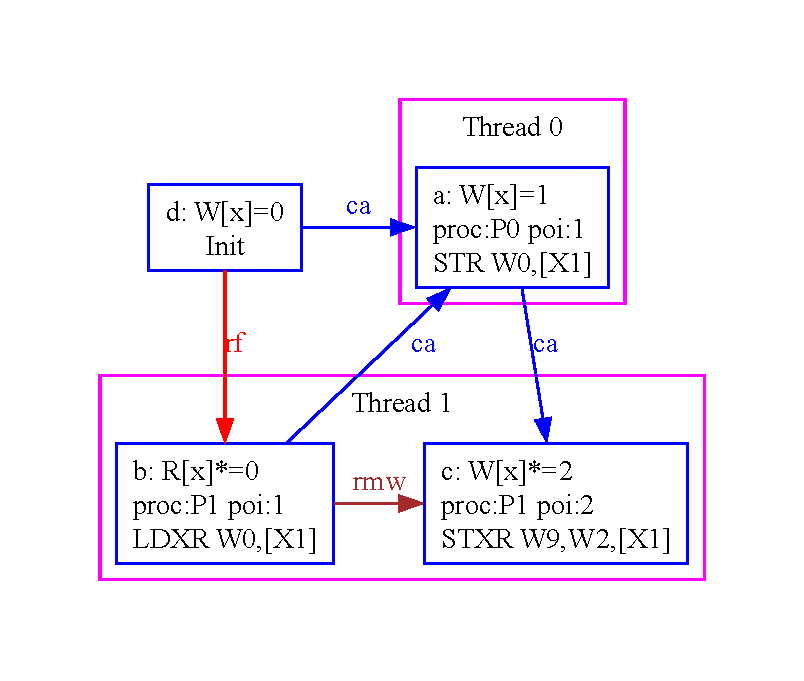
\includegraphics[
    max width=0.6\linewidth
  ]{figures/rmw-ldxr-stxr.dot-crop.pdf}
  \caption{A candidate execution for \texttt{rmw-ldxr-stxr}.}
  \label{fig:rmw-ldxr-stxr-candidate}
\end{figure}

Figure~\ref{fig:rmw-ldxr-stxr-candidate} shows this candidate
execution graphically.
%
This candidate execution is architecturally Forbidden.
Effects that are generated by a successful Load-Exclusive/Store-Exclusive pair, 
as is the case in test rmw-ldxr-stxr above, or an atomic instruction such as a CAS, are required to appear to be atomic.  
 
The typical shape is as follows: 
\begin{itemize}
\item A Memory Read Effect of a Location x 
\item A Memory Write Effect of the same Location x 
\item The Read Effect and the Write Effect are related by the “Read-modify-write” relation, which indicates that the Effects are either: 
  \begin{itemize}
  \item Generated by a Load-Exclusive instruction for
  the Read, and by a corresponding Store-Exclusive
  instruction for the Write, forming a successful
  pair; or 
  \item Generated by the same atomic instruction, for
  example a CAS.
  \end{itemize}
\end{itemize}

This requirement means that it must not be possible
for an intervening Write Effect of the same Location
such as the Effect (a) generated by STR W4,[X1], to
happen in between the Read Effect (b) and the Write
Effect (c) of the Read-modify-write pair. 

% Requirement 7 (rewritten)
This places a requirement on the hardware that if the Memory Write Effect (a)
is Coherence-after the Memory Read Effect (b) but Coherence-before the Memory
Write Effect (c), then the hardware is not architecturally Allowed to let
Effect (b) and Effect (c) form a successful Read-Modify-Write pair.
%
Specifically, the execution of the Load-Exclusive (b) transitions the
Exclusives monitor to the Exclusive Access state. However, the execution of the
Store (a) in P0 causes the Exclusives monitor to transition into the Open
Access state and therefore the attempted execution of the Store-Exclusive (c)
fails.

In most cases, this work can be done exclusively within the PE P1 using a
signal (e.g. snoop request) sent by the system to PE P1 in response to the
Write Effect (a). The signal can be used to transition the global monitor in
P1. If the global monitor is located outside of P1 in the system, then the
system machinery would be responsible for transitioning P1’s global monitor
upon processing the Write Effect (a).  
 
As a consequence, the test in Figure~\ref{fig:litmus-rmw-cas}, where the
Load-Exclusive/Store-Exclusive pair has been replaced by an atomic CAS
instruction, is also architecturally Forbidden.
\litmusinputwithlink[fig:litmus-rmw-cas]{rmw-cas}

\begin{figure}[!htbp]
  \centering
  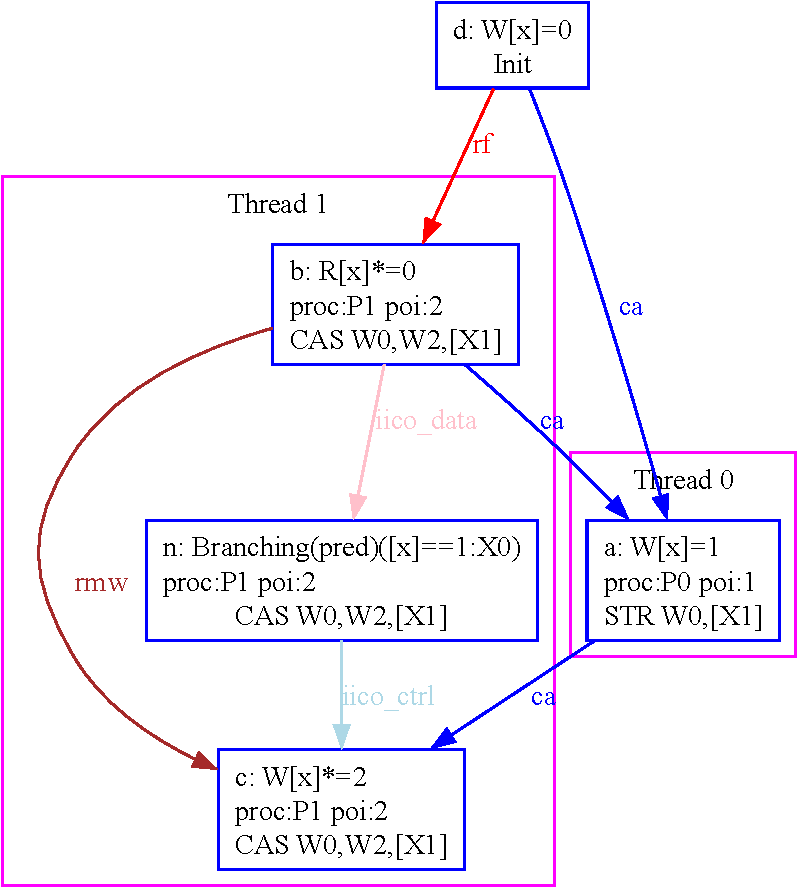
\includegraphics[
    max width=0.7\linewidth
  ]{figures/rmw-cas-crop.pdf}
  \caption{A candidate execution for \texttt{rmw-cas}.}
  \label{fig:rmw-cas-candidate}
\end{figure}

Figure~\ref{fig:rmw-cas-candidate} shows the corresponding
architecturally Forbidden execution graphically.
% Requirement 8 (rewritten)
This places a requirement on the hardware that if the Memory Write Effect (a)
is Coherence-after the Memory Read Effect (b) but Coherence-before the Memory
Write Effect (c), then the hardware is not architecturally Allowed to let
Effect (b) and Effect (c) form a successful Read-Modify-Write pair.
%
Specifically, as Effect (b) is generated by the same atomic instruction that
generated Effect (c), the hardware must re-perform Effect (b), because it must
ensure that the Read Effect (b) Reads-from the Write Effect (a).

\chapter{A Collection of Concurrent Scenarios}
\label{chap:concurrent-scenarios}

This chapter aims to: 
\begin{itemize}
\item Provide a reference point for naming schemes used in concurrent scenarios, typically represented as litmus tests; 
\item List a number of classic, standard, interesting or notable litmus tests. 
\end{itemize}

\section{Naming schemes}

Concurrent scenarios represented as litmus tests have names whose meaning is not immediately evident.  
%
This is partly due to the use of acronyms such as ``WRC'', which stands for
``Write-to-Read-Causality'', as shown in Figure~\ref{fig:litmus-wrc}.
\litmusinputwithlink[fig:litmus-wrc]{WRC}

The WRC test in Figure~\ref{fig:litmus-wrc} does not have any synchronisation (e.g. barriers,
dependencies, Relaxed or Acquire...). A classic way of designating a variation
of a known shape, such as WRC, equipped with synchronisation, is to augment the
name of the test by listing the type of synchronisation involved in the test,
separating the threads involved with a ``+'' sign.  
 
For example, WRC+rel+addr is the name of a sibling of WRC equipped with a
Release Store on the second thread and an address dependency on the third
thread, as shown in Figure~\ref{fig:litmus-wrc-rel-addr}.
\litmusinputwithlink[fig:litmus-wrc-rel-addr]{WRC+rel+addr}

This note aims to list most common concurrent scenarios, their full names and their acronyms. 
 
Certain classic concurrent scenarios have alphanumeric names which are not acronyms, such as “R”, “S” or “Z6.3”. These names are simply due to arbitrary naming choices made the inventors of these tests, without any a priori intent for these names to come to posterity. But some of these arbitrary names have become relatively standard in the literature all the same.  

Sometimes litmus tests do not have standard names (whether acronyms or arbitrary alphanumeric names) in the literature. In this case, a somewhat common naming scheme is to compose the name of the test by listing the type of Effects involved in the test, separating the threads involved with a ``+'' sign. For example, ``W+RW+RR'' is the name of a 3-threaded test such that: 
\begin{itemize}
\item The first thread has a Store instruction which generates an Explicit Memory Write Effect (symbolised by the W before the first “+” sign); 
\item The second thread has a Load instruction, which generates an Explicit Memory Read Effect (symbolised by the R after the first “+” sign), in program order before a Store instruction which generates an Explicit Memory Write Effect (symbolised by the W before the second “+” sign); 
\item The third thread has a Load instruction, which generates an Explicit Memory Read Effect (symbolised by the R after the second “+” sign), in program order before another Load instruction, which generates an Explicit Memory Read Effect (symbolised by the R at the end) 
\end{itemize}

In other words, “W+RW+RR” is another name for the WRC test, as shown in Figure~\ref{fig:litmus-w-rw-rr}.
\litmusinputwithlink[fig:litmus-w-rw-rr]{W+RW+RR}

\section{``Coherence'' scenarios}

This section illustrates litmus tests for ``SC-per-location'' or ``Coherence''
(coXY) scenarios, i.e. coXY litmus tests where X and Y are in \{R,W\}.

\subsection{coWW litmus test}

\diygenoneloc{coWW}{PosWW Coe}

\litmusinputwithlink[fig:litmus-coww-2]{coWW}

\litmustodesc{coWW}

\subsection{coRW1 litmus test}

\diygenoneloc{coRW1}{PosRW Rfe}

\litmusinputwithlink[fig:litmus-corw1-2]{coRW1}

\litmustodesc{coRW1}

\subsection{coRW2 litmus test}

\diygenoneloc{coRW2}{PosRW Coe Rfe}

\litmusinputwithlink[fig:litmus-corw2]{coRW2}

\litmustodesc{coRW2}

\subsection{coWR litmus test}

\diygenoneloc{coWR}{PosWR Fre}

\litmusinputwithlink[fig:litmus-cowr-2]{coWR}

\litmustodesc{coWR}

\subsection{coRR litmus test}

\diygenoneloc{coRR}{PosRR Fre Rfe}

\litmusinputwithlink[fig:litmus-corr-2]{coRR}

\litmustodesc{coRR}

\section{Load buffering (LB) scenarios}

\subsection{LB litmus test}

\diygen{LB}{PodRW Rfe PodRW Rfe}
\litmusinputwithlink[fig:litmus-lb]{LB}

\litmustodesc{LB}

\subsection{R+WW+RW litmus test}

R+WW+RW is a 3-threaded variant of LB.

\diygen{R+WW+RW}{Fre PodWW Rfe PodRW Rfe}

\litmusinputwithlink[fig:litmus-r-ww-rw]{R+WW+RW}

\litmustodesc{R+WW+RW}

\subsection{R+WR+W+RW litmus test}

R+WR+W+RW is a 4-threaded variant of LB.

\diygen{R+WR+W+RW}{Fre PodWR Fre Rfe PodRW Rfe}

\litmusinputwithlink[fig:litmus-r-wr-w-rw]{R+WR+W+RW}

\litmustodesc{R+WR+W+RW}

\section{MP, WRC, and ISA2 scenarios}

This section illustrates litmus tests for the Message passing (MP),
Write-to-Read-Causality (WRC) and ``ISA2'' scenarios.

\subsection{MP litmus test}

\diygen{MP}{PodWW Rfe PodRR Fre}

\litmusinputwithlink[fig:litmus-mp-2]{MP}

\litmustodesc{MP}

\subsection{WRC litmus test}

WRC is a 3-threaded variant of MP.

\diygen{WRC}{Rfe PodRW Rfe PodRR Fre}

\litmusinputwithlink[fig:litmus-wrc-2]{WRC}

\litmustodesc{WRC}

\subsection{ISA2 litmus test}

ISA2 is another 3-threaded variant of MP.

Called thus because it was the second (of two) litmus test in the Power ISA manual.

\diygen{ISA2}{PodWW Rfe PodRW Rfe PodRR Fre}

\litmusinputwithlink[fig:litmus-isa2]{ISA2}

\litmustodesc{ISA2}

\subsection{W+RR+WR+WR}

W+RR+WR+WR is a 4-threaded variant of MP.

\diygen{W+RR+WR+WR}{Rfe PodRR Fre PodWR Fre PodWR Fre}

\litmusinputwithlink[fig:litmus-w-rr-wr-wr]{W+RR+WR+WR}

\litmustodesc{W+RR+WR+WR}

\section{RSW, RDW, and PPOxy scenarios}

This section illustrates litmus tests for the Read-Same-Write (RSW),
Read-Different-Writes (RDW), and PPOxy scenarios. That is, variations of the
reading side of MP. In PPOxy scenarios, x and y range over \{A,D,C\}, with `A'
standing for Address Dependency, `D' standing for Data Dependency, and `C'
standing for Control Dependency.

\subsection{PPOAA litmus test}

\diygen{PPOAA}{PodWW Rfe DpAddrdW Rfi DpAddrdR Fre}

\litmusinputwithlink[fig:litmus-ppoaa]{PPOAA}

\litmustodesc{PPOAA}

\subsection{PPODA litmus test}

\diygen{PPODA}{PodWW Rfe DpDatadW Rfi DpAddrdR Fre}

\litmusinputwithlink[fig:litmus-ppoda]{PPODA}

\litmustodesc{PPODA}

\subsection{PPOCA litmus test}

\diygen{PPOCA}{PodWW Rfe DpCtrldW Rfi DpAddrdR Fre}

\litmusinputwithlink[fig:litmus-ppoca]{PPOCA}

\litmustodesc{PPOCA}

\subsection{PPOAC litmus test}

\diygen{PPOAC}{PodWW Rfe DpAddrdW Rfi DpCtrldR Fre}

\litmusinputwithlink[fig:litmus-ppoac]{PPOAC}

\litmustodesc{PPOAC}

\subsection{PPODC litmus test}

\diygen{PPODC}{PodWW Rfe DpDatadW Rfi DpCtrldR Fre}

\litmusinputwithlink[fig:litmus-ppodc]{PPODC}

\litmustodesc{PPODC}

\subsection{PPOCC litmus test}

\diygen{PPOCC}{PodWW Rfe DpCtrldW Rfi DpCtrldR Fre}

\litmusinputwithlink[fig:litmus-ppocc]{PPOCC}

\litmustodesc{PPOCC}

\subsection{PPO\{DD,CD\} litmus test}

The PPODD and PPOCD litmus test do not exist, because there cannot be a Data
dependency to a Memory Read Effect.

\subsection{RSW litmus test}

\diygen{RSW}{PodWWPL RfeLP DpAddrdR PosRR DpAddrdR Fre}

\litmusinputwithlink[fig:litmus-rsw]{RSW}

\litmustodesc{RSW}

\subsection{RDW litmus test}

\diygen{RDW}{PodWW L Rfe DpAddrdR FrLeave RfBack DpAddrdR Fre}

\litmusinputwithlink[fig:litmus-rdw]{RDW}

\litmustodesc{RDW}

\section{SB, RWC, IRIW, etc.}

This section illustrates litmus tests for the Store buffering (SB),
Read-to-Write Causality (RWC), Independent Reads of Independent Writes (IRIW)
and related scenarios.

\subsection{SB litmus test}

\diygen{SB}{PodWR Fre PodWR Fre}

\litmusinputwithlink[fig:litmus-sb]{SB}

\litmustodesc{SB}

\subsection{RWC litmus test}

RWC is a 3-threaded variant of SB.

\diygen{RWC}{Rfe PodRR Fre PodWR Fre}

\litmusinputwithlink[fig:litmus-rwc]{RWC}

\litmustodesc{RWC}

\subsection{IRIW litmus test}

IRIW is a 3-threaded variant of SB.

\diygen{IRIW}{Rfe PodRR Fre Rfe PodRR Fre}

\litmusinputwithlink[fig:litmus-iriw]{IRIW}

\litmustodesc{IRIW}

\section{“S” and Write-to-Write-Causality (WWC) scenarios}

\subsection{S litmus test}

\diygen{S}{PodWW Rfe PodRW Coe}

\litmusinputwithlink[fig:litmus-s]{S}

\litmustodesc{S}

\subsection{WWC litmus test}

WWC is a 3-threaded variant of S.

\diygen{WWC}{Rfe PodRW Rfe PodRW Coe}

\litmusinputwithlink[fig:litmus-wwc]{WWC}

\litmustodesc{WWC}

\subsection{W+WR+RR+W}

W+WR+RR+W is a 4-threaded variant of S.

\diygen{W+WR+RR+W}{Rfe PodRW Rfe PodRR Fre Coe}

\litmusinputwithlink[fig:litmus-w-wr-rr-w]{W+WR+RR+W}

\litmustodesc{W+WR+RR+W}

\section{``R'' scenarios}

\subsection{R litmus test}

\diygen{R}{PodWW Coe PodWR Fre}

\litmusinputwithlink[fig:litmus-r]{R}

\litmustodesc{R}

\subsection{W+RW+WR litmus test}

W+RW+WR is a 3-threaded variant of R.

\diygen{W+RW+WR}{Rfe PodRW Coe PodWR Fre}

\litmusinputwithlink[fig:litmus-w-rw-wr]{W+RW+WR}

\litmustodesc{W+RW+WR}

\subsection{W+RR+2W litmus test}

W+RR+2W is another 3-threaded variant of R.

\diygen{W+RR+2W}{Rfe PodRR Fre PodWW Coe}

\litmusinputwithlink[fig:litmus-w-rr-2w]{W+RR+2W}

% call your tool, spit out latex, include here
% This English narration of the litmus test XXX can be generated using: \texttt{~/bin/litmustodesc test... }
% English narration

\litmustodesc{W+RR+2W}

\subsection{W+RR+WR+WW }

W+RR+WR+WW is a 4-threaded variant of R.

\diygen{W+RR+WR+WW}{Rfe PodRR Fre PodWR Fre PodWW Coe}

\litmusinputwithlink[fig:litmus-w-rr-wr-ww]{W+RR+WR+WW}

\litmustodesc{W+RR+WR+WW}

\section{``2+2w'' scenarios}

\subsection{2+2w litmus test}

\diygen{2+2w}{PodWW Coe PodWW Coe}

\litmusinputwithlink[fig:litmus-2-2w]{2+2w}

\litmustodesc{2+2w}

\subsection{W+RW+2W litmus test }

W+RW+2W can be seen as the 2+2W scenario spread across 3 threads.

\diygen{W+RW+2W}{Rfe PodRW Coe PodWW Coe}

\litmusinputwithlink[fig:litmus-w-rw-2w]{W+RW+2W}

\litmustodesc{W+RW+2W}

\subsection{W+RW+W+RW litmus test}

W+RW+W+RW can be seen as the 2+2W scenario spread across 4 threads.

\diygen{W+RW+W+RW}{Rfe PodRW Coe Rfe PodRW Coe}

\litmusinputwithlink[fig:litmus-w-rw-w-rw]{W+RW+W+RW}

\litmustodesc{W+RW+W+RW}

\section{``Z6'' scenarios}

\subsection{Z6.3 litmus test}

\diygen{Z6.3}{PodWW Coe PodWW Rfe PodRR Fre}

\litmusinputwithlink[fig:litmus-z6-3]{Z6.3}

\litmustodesc{Z6.3}

\bibliographystyle{plainurl}
\bibliography{references}

\end{document}
